\documentclass[conference]{IEEEtran}

\usepackage{amsmath,amssymb}
\usepackage{graphicx}
\usepackage{lmodern}
\usepackage{tgtermes}
\usepackage{url}

\title{Cost-Selected Parallel Decoding of Sector--Disk Erasure Codes on CPUs and GPUs}

\author{\IEEEauthorblockN{Tejas Singh Sodhi, Arnav Verma, Advay Satish, and Dhanush Kumar}
\IEEEauthorblockA{Birla Institute of Technology and Science, Pilani\\
K K Birla Goa Campus, Goa, India}}

\begin{document}
\maketitle

\begin{abstract}
Erasure-code recovery reconstructs missing storage sectors by applying finite-field equations to surviving data. This paper evaluates CPU and CUDA decoders for Sector--Disk codes, which protect against complete-disk and additional sector failures. The decoders select between applying matrices to data in sequence, multiplying coefficient matrices first, and partitioning independent failure groups. CPU optimization combines single-instruction multiple-data (SIMD) arithmetic with OpenMP; GPU variants use direct or table-based multiplication. An initial layer study achieves 1.69$\times$--34.85$\times$ the scalar sequential baseline at eight threads. A final 900-trial experiment compares one, two, four, and eight CPU threads with both GPU variants, using shuffled trial order and 8--128 MiB stripes. At 32 MiB, the table-based RTX 4050 decoder is 1.25$\times$--1.39$\times$ faster than the best tested CPU setting for GF($2^{32}$), including transfers and setup, but slower for the smaller fields. At 128 MiB, the CPU wins the tested GF($2^{32}$) case. Profiles identify region arithmetic, GF($2^{32}$) table construction, transfers, and synchronization as targets. An extended 23,028-trial study focuses on how the GPU's advantage changes with CPU parallelism. For GF($2^{32}$) its lead falls from 1.70$\times$--2.12$\times$ at one CPU thread to 1.25$\times$--1.40$\times$ at two to four, and at 128 MiB the CPU overtakes it at $T\approx2.3$. On a hybrid i5-13420H, gPPM scaling peaks at exactly four threads, the number of performance cores, where the projected GPU lead reaches parity. Efficiency cores restore a 2.5$\times$--2.9$\times$ GPU lead. An ablation attributes a 5.93$\times$ geometric-mean speedup to the combined layers, and reproductions confirm the original paper's parameter trends. These results favor workload-specific thread and backend selection over assuming that more parallelism always improves recovery.
\end{abstract}

\begin{IEEEkeywords}
erasure coding, Sector--Disk codes, gPPM, OpenMP, SIMD, CUDA, recovery
\end{IEEEkeywords}

\section{Introduction}
Erasure codes store data with parity so that missing sectors can be reconstructed without keeping full replicas. Recovery solves finite-field equations over the surviving data, and applying those equations to large regions can make computation a significant part of repair time. This study focuses on Sector--Disk (SD) codes, which tolerate both complete-disk failures and additional sector failures. Their parity-check equations include row-local relationships as well as equations spanning the whole stripe; this structure means some failed sectors can be recovered independently while others depend on those results \cite{li2023gppm}.

Prior work provides two ways to exploit this structure. Partitioned and Parallel Matrix (PPM) recovery separates independent failure groups and processes them concurrently \cite{li2015ppm}. Generalized PPM (gPPM) also selects between two equivalent calculation orders: first applying the parity-check matrices to data regions, or first multiplying the smaller coefficient matrices \cite{li2023gppm}. Single-instruction multiple-data (SIMD) instructions accelerate the finite-field operations within each region \cite{plank2013simd}.

This paper asks how much these optimizations contribute to an SD decoder, where execution time and instruction work concentrate, and when GPU offloading beats the best tested CPU thread count. An initial CPU-layer study isolates cumulative implementation gains. The final experiment then compares four CPU thread settings with two CUDA variants in shuffled order, measures stripe-size scaling, and profiles recovery-only ranges. At 32 MiB, the table GPU beats the best tested CPU setting in GF($2^{32}$), but the CPU wins the tested 128 MiB case. An extended evaluation (Section~\ref{sec:gpu-threads}) asks exactly where the GPU's advantage disappears as CPU threads are added, where CPU speedup tapers off, which optimization layers matter, and whether the original paper's results reproduce. The contribution is a reproducible implementation, bottleneck analysis, and evaluation on one CPU/GPU system plus a second hybrid CPU, rather than a new code construction or distributed-scaling algorithm.

\section{Background and Related Work}
\subsection{SD-code recovery}
An SD code has $n$ disks, $r$ sector rows per disk, tolerates $m$ disk failures and $s$ additional sector failures, and uses the finite field $GF(2^w)$ of $w$-bit symbols. A stripe is the $nr$ sectors protected together; $z$ counts rows with additional sector failures. Its parity-check matrix $H$ has $mr+s$ rows. A valid stripe $B$ satisfies $HB=0$. Let $F,S$ contain the failed and surviving columns, and $B_F,B_S$ the corresponding data. For an invertible $F$,
\begin{equation}
B_F = F^{-1} S B_S.
\label{eq:recover}
\end{equation}
The normal sequence computes $S B_S$ before applying $F^{-1}$. Matrix-first computes $G=F^{-1}S$ first, then applies $G$ to the surviving data. Both recover the same sectors, but their data-region operation counts can differ \cite{li2023gppm}. SD parity equations include both row-local and stripe-wide constraints. PPM uses the row-local structure to identify independent failure groups, then recovers the coupled remainder \cite{li2015ppm}.

\subsection{Positioning among prior optimizations}
PPM introduced matrix partitioning for asymmetric codes; gPPM extended it with per-matrix sequence selection that accounts for both nonzero and non-one coefficients \cite{li2015ppm,li2023gppm}. SIMD finite-field kernels accelerate each region operation and complement this reduction in work \cite{plank2013simd}. This study keeps the SD code and parity equations fixed, and optimizes the recovery schedule and arithmetic kernels.

\section{Recovery Design}
\subsection{Cost model and selection}
For a coefficient matrix $M$, let $u(M)$ count nonzero entries and $v(M)$ count entries greater than one. A region multiply-XOR multiplies each source symbol by a field coefficient and XORs it into a destination; coefficient one requires only XOR. The estimated cost is
\begin{equation}
  C(M)=u(M)+c\,v(M),
\label{eq:cost}
\end{equation}
where $c$ estimates the additional relative cost of a non-one multiply-XOR compared with a coefficient-one XOR. For the normal and matrix-first sequences,
\begin{align}
 C_{\mathrm{normal}} &= u(S)+u(F^{-1})+c[v(S)+v(F^{-1})],\\
 C_{\mathrm{matrix}} &= u(F^{-1}S)+c\,v(F^{-1}S).
\end{align}
For PPM, the decoder sums the cheaper sequence estimate for each independent group and the remainder. It uses this partition only when its estimated cost is lower than the cheaper whole-matrix sequence. The model estimates arithmetic work, not scheduling overhead or elapsed time.

The decoder estimates $c$ per field and build by timing coefficient-one and coefficient-two operations on 256 KiB regions. It uses the multiply-XOR/XOR time ratio minus one, clamped at zero. Since this calibration is hardware-dependent, $c$ can change sequence selection across platforms.

\subsection{Partitioned and parallel execution}
Rows with exactly $m$ failed sectors have enough row-local equations to recover them independently. The decoder prepares these groups and a remainder containing the other row-local and all stripe-wide equations. OpenMP workers recover disjoint groups; a barrier ensures those outputs are ready before the remainder is decoded. The team size is capped at the number of independent groups.

The final optimization also splits the remainder's data regions into symbol-aligned byte ranges. Workers apply the same matrix-vector transformation to disjoint output ranges, avoiding write conflicts.

\subsection{SIMD region kernels}
The SIMD build dispatches at runtime with a scalar fallback. GF($2^8$) uses SSSE3 byte shuffles and nibble tables (16 bytes per vector); GF($2^{16}$) and GF($2^{32}$) use AVX2 gathers and byte-contribution tables (eight symbols per vector). The scalar comparison uses the same M3 code with SIMD disabled.

\subsection{CUDA recovery}
The GPU decoder retains matrix preparation and sequence selection on the host. Each CUDA thread computes one output field symbol, accumulating all nonzero coefficient contributions in a register. Adjacent threads process adjacent symbols, and one kernel evaluates a matrix-vector product rather than launching a kernel for each coefficient. Normal recovery needs two products; matrix-first needs one. Independent groups use separate streams and scratch buffers, and finish before the remainder starts. Each recovery transfers the stripe to the device once and copies the result back once.

The GPU scalar variant uses direct shift-and-reduce field multiplication. The table variant uses logarithm/antilogarithm tables for GF($2^8$) and GF($2^{16}$), and split-byte tables for GF($2^{32}$). Both execute many CUDA threads; ``scalar'' describes reference arithmetic, not serial GPU execution. Each variant calibrates its cost weight using sixteen interleaved coefficient-one/coefficient-two probe pairs after warm-up, each on 32,768 symbols. This is a heuristic: the fixed coefficient and restricted probe values do not represent every coefficient or data distribution, especially for split-byte multiplication.

\begin{table}[t]
\caption{CPU decoder layers in the performance comparison.}
\label{tab:layers}
\centering
\footnotesize
\begin{tabular}{c p{0.76\columnwidth}}
\hline
Layer & Decoder configuration \\
\hline
L0 & Scalar normal recovery; single-threaded reference \\
L1 & Scalar cost selection; parallel groups, serial remainder \\
L2 & L1 with SIMD region kernels \\
L3 & L2 with parallel byte ranges in the remainder \\
\hline
\end{tabular}
\end{table}

\begin{figure*}[t]
\centering
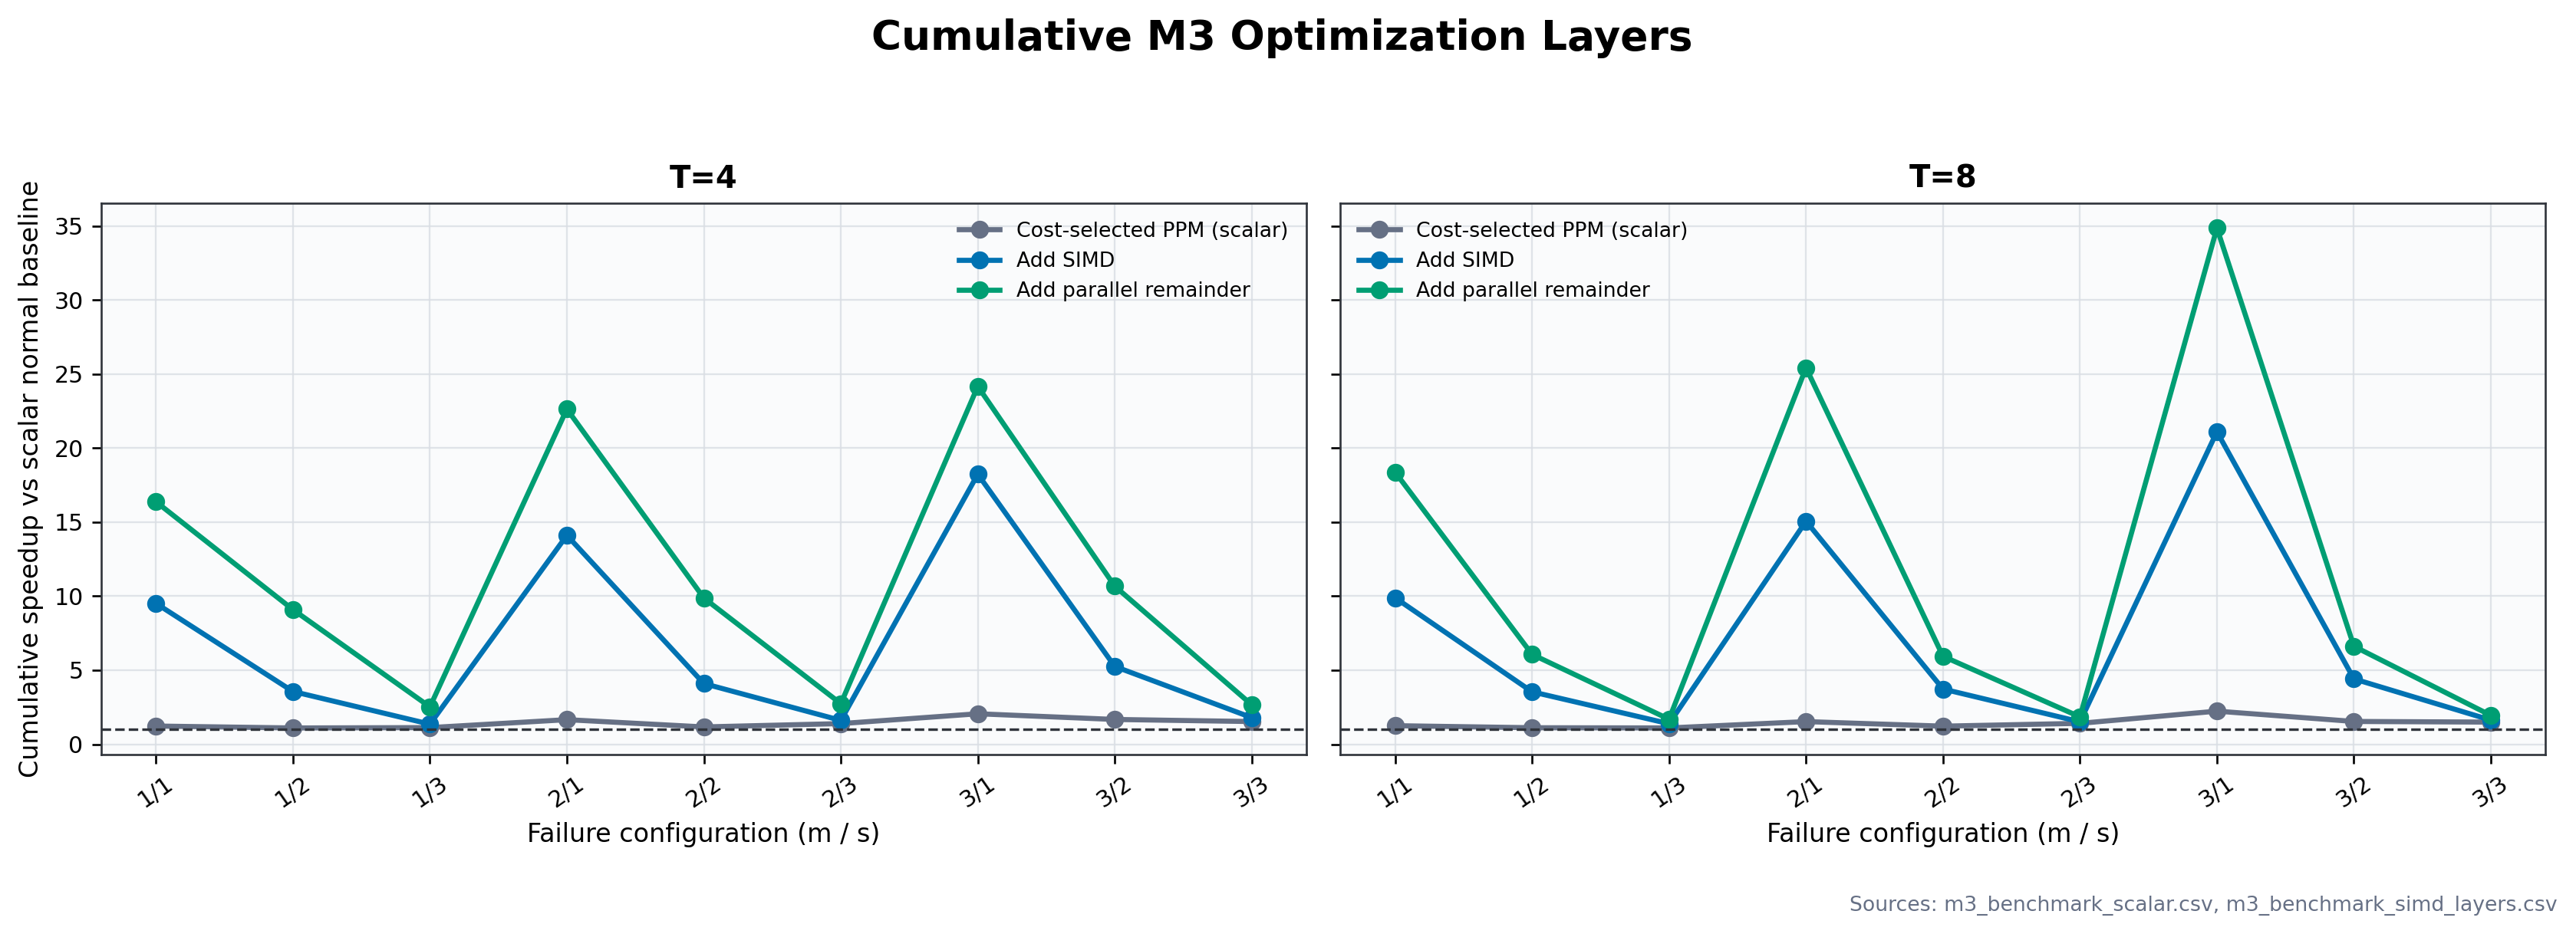
\includegraphics[width=0.88\textwidth]{../../results/milestone3/m3_cumulative_speedup.png}
\caption{Cumulative median speedup at T=4 and T=8 relative to scalar normal recovery. Curves show cost-selected scalar PPM, SIMD PPM, and SIMD PPM with a parallel remainder.}
\label{fig:layers}
\end{figure*}

\begin{table*}[t]
\caption{Single-threaded L0 median time and speedups of L1--L3 at T=8, each calculated as L0 time divided by layer time.}
\label{tab:times}
\centering
\small
\setlength{\tabcolsep}{8pt}
\renewcommand{\arraystretch}{1.15}
\begin{tabular}{cc l rrrr}
\hline
$m$ & $s$ & Field & L0 (ms) & L1 speedup & L2 speedup & L3 speedup\\
\hline
1&1&GF($2^8$) &36.031&1.25$\times$&9.89$\times$&\textbf{18.37$\times$}\\
1&2&GF($2^{16}$)&55.211&1.11$\times$&3.54$\times$&\textbf{6.07$\times$}\\
1&3&GF($2^{32}$)&45.913&1.10$\times$&1.38$\times$&\textbf{1.69$\times$}\\
2&1&GF($2^8$) &65.968&1.53$\times$&15.06$\times$&\textbf{25.42$\times$}\\
2&2&GF($2^{16}$)&82.134&1.22$\times$&3.73$\times$&\textbf{5.94$\times$}\\
2&3&GF($2^{32}$)&60.146&1.41$\times$&1.51$\times$&\textbf{1.85$\times$}\\
3&1&GF($2^8$) &99.343&2.23$\times$&21.10$\times$&\textbf{34.85$\times$}\\
3&2&GF($2^{16}$)&111.524&1.54$\times$&4.41$\times$&\textbf{6.61$\times$}\\
3&3&GF($2^{32}$)&74.373&1.49$\times$&1.63$\times$&\textbf{1.94$\times$}\\
\hline
\end{tabular}
\end{table*}

\section{Experimental Method}
\subsection{Platform and workloads}
Measurements use an Intel Core Ultra 9 185H and GCC 11.4.0 with \texttt{-O2 -fopenmp}. We test all nine $(m,s)\in\{1,2,3\}^2$ pairs at $n=r=16$, $z=1$, on a 32 MiB stripe (256 sectors of 128 KiB). For $s=1,2,3$, the fields are GF($2^8$), GF($2^{16}$), and GF($2^{32}$). Each configuration has one warm-up and ten timed recovery trials; fault injection, validation, checksums, and CSV output are excluded.

Published coefficients come from Plank's SD implementation \cite{plank2013software}. Timed failures erase disks $0,\ldots,m-1$ and sectors in row zero at columns $m,\ldots,m+s-1$, exposing 15 independent groups. Field width and sector-failure tolerance vary together; cross-field results therefore do not isolate field width alone. The previous milestone used fixed matrix-first recovery for independent groups and a normal, serial remainder.

GPU tests use an RTX 4050 Laptop GPU with 6 GB memory, driver 580.178.04, and CUDA 13.0.88 compiled with \texttt{-O2}. An initial 270-trial GPU check used an eight-thread CPU comparator. The final benchmark replaces that restricted comparison with CPU L3 at $T=1,2,4,8$ and both GPU variants, sharing encoded bytes and failures within each configuration. It runs all nine workloads at 32 MiB (540 trials), and $m=2$, $s=1,2,3$ at 8 and 128 MiB (180 trials each). Each variant warms once; a seeded shuffle changes variant order in each of ten timed rounds. OpenMP dynamic teams are disabled, with default OS scheduling and no explicit affinity. The per-field heuristic calibration is cached after warm-up.

Table~\ref{tab:layers} defines the four CPU layers; $T$ is the requested OpenMP thread count. L0--L1 use the scalar build; L2--L3 use the SIMD build, so L2/L1 compares complete decoders. Cumulative speedup is the L0 median divided by a layer median; incremental gain is the previous layer's median divided by the current layer's.

\subsection{Correctness and reported metrics}
Timed trials must match the saved bytes and checksum and have zero syndrome, meaning every parity equation is satisfied. The CPU sweep tests one deterministic failure layout per feasible published parameter/$z$ point, using 16-byte sectors rather than the 128 KiB timed sectors. It covers $n,r=4,\ldots,24$, $m,s=1,2,3$, and $z=1,\ldots,s$, but not every failure placement. Large-buffer SIMD behavior is checked separately in unit tests and timed recoveries.

Logical region-operation counts describe algorithmic work. Serial CPU paths count calls; parallel remainder and GPU paths derive counts from matrix nonzeros. The checks establish cross-thread consistency and agreement with each variant's warm-up count, not independent measurement of every executed operation. Useful-data throughput is non-parity bytes divided by recovery time; speedups use ratios of median end-to-end times.

GPU end-to-end timing includes host matrix preparation, device allocation, table and stripe transfers, launches, synchronization, and cleanup. Buffers and tables are recreated per recovery; CUDA startup and cost calibration occur during warm-up. Summed per-kernel CUDA-event durations are also recorded. Because streams overlap, that sum may exceed wall-clock recovery time and cannot be subtracted from it to estimate transfer time.

Final latency is the median of ten native trials. Thread speedup is $t_{\mathrm{L3},1}/t_{\mathrm{L3},T}$; efficiency divides this speedup by $T$. The CPU comparator for offload is the lowest median among the four tested settings, not an exhaustive hardware-tuned optimum. For example, the 25th--75th percentile range for the two-thread $(m,s)=(2,3)$ CPU case is 19.90--28.58 ms at 8 MiB and 31.29--37.36 ms at 32 MiB. All interquartile ranges are retained; they describe within-run variation, not confidence intervals.

\subsection{Profiling protocol}
Profiling is separate from native timing. Callgrind 3.18.1 records recovery-only CPU instructions at $T=1$, $m=2$, and each field, with 32 MiB stripes. Encoding, warm-up, fault injection, and validation are outside the instrumented range. A profiling-only linker wrapper freezes the corresponding native calibration weight, preventing emulation overhead from changing sequence selection. Each profile's logical operation count matches its native counterpart. Function self costs include instructions attributed to inlined intrinsic headers; instruction shares are not elapsed-time shares.

Nsight Systems 2025.3.2 traces one warmed recovery for each GPU variant and field at the same parameters. CUDA profiler start/stop calls bound capture; CPU sampling is disabled. We report the union of kernel intervals across streams, actual device-copy durations, and host API durations. These categories overlap and are not an additive latency decomposition. Hardware counters through Linux \texttt{perf} are unavailable under the machine's permission settings, so cache-miss rates, bandwidth saturation, and occupancy are not inferred.

\begin{table}[t]
\caption{Nsight recovery traces at $m=2$, 32 MiB. Kernel union, summed device-copy intervals, stream-synchronization API time, and allocation/free API time are in ms and may overlap. One profiled run per row.}
\label{tab:gpu-profile}
\centering
\footnotesize
\setlength{\tabcolsep}{3pt}
\begin{tabular}{clrrrrr}
\hline
$w$ & Variant & Kernels & Kernel & Copy & Sync & Alloc/free\\
\hline
8&Direct&32&23.97&9.31&23.43&2.90\\
8&Table&17&18.56&8.93&18.29&1.99\\
16&Direct&32&18.57&9.27&18.09&2.81\\
16&Table&32&23.59&9.42&23.13&3.58\\
32&Direct&32&17.11&9.03&16.55&2.77\\
32&Table&17&11.80&10.12&11.53&2.17\\
\hline
\end{tabular}
\end{table}

\section{Results}
\subsection{Correctness}
All 7,833 feasible CPU parameter-grid points pass; 105 of 7,938 parameter/$z$ combinations are infeasible. At $T=1$ and $T=4$, recovered bytes, syndromes, and operation counts agree. All 720 CPU-layer trials pass validation. Separate GPU tests pass 12 direct/two-stage matrix checks and 64 small-stripe recoveries across all fields and both variants. NVIDIA Compute Sanitizer reports zero memory errors. All 270 initial CPU/GPU trials and all 900 final benchmark trials pass byte equality, checksum, and zero-syndrome checks. The GPU tests do not reproduce the full CPU parameter-grid sweep.

\subsection{Layered performance}
Fig.~\ref{fig:layers} compares the optimization layers; Table~\ref{tab:times} gives their cumulative T=8 speedups and baseline times.

L1 improves all nine cases by 1.10$\times$--2.23$\times$ over L0. SIMD gives its largest gain in GF($2^8$): L2 reaches 21.10$\times$ over L0 and up to 9.85$\times$ over L1. In GF($2^{32}$), L2 improves on L1 by 1.07$\times$--1.26$\times$. Parallel remainder processing adds 1.20$\times$--1.86$\times$ over L2 in every T=8 case. Final speedups range from 1.69$\times$ to 34.85$\times$.

\subsection{Final thread and size scaling}
Fig.~\ref{fig:scaling} shows the final same-run CPU scaling. Relative to L3 at one thread, the best tested setting achieves 1.37$\times$--2.90$\times$ at 32 MiB. Eight threads win all three GF($2^8$) cases, but two or four win five of the six wider-field cases. For example, at $(m,s)=(2,3)$, two threads take 32.12 ms and eight take 37.49 ms. This differs from the earlier fixed-order layer study: scheduling, calibration, and system variation can affect rankings. Gains over L2 at a fixed thread count must not be confused with gains from increasing the thread count.

Fig.~\ref{fig:sizes} compares stripe sizes at $m=2$. For GF($2^{32}$), the best tested CPU takes 21.88, 32.12, and 59.47 ms at 8, 32, and 128 MiB; the table GPU takes 8.47, 24.48, and 83.26 ms. Thus its speedup over the best tested CPU changes from 2.58$\times$ to 1.31$\times$ to 0.71$\times$. Sizes ran in the fixed order 32, 8, then 128 MiB in separate processes with fresh calibration. System state, run order, and variable thread selection confound these one-session observations; they do not establish a general crossover threshold.

\begin{figure*}[t]
\centering
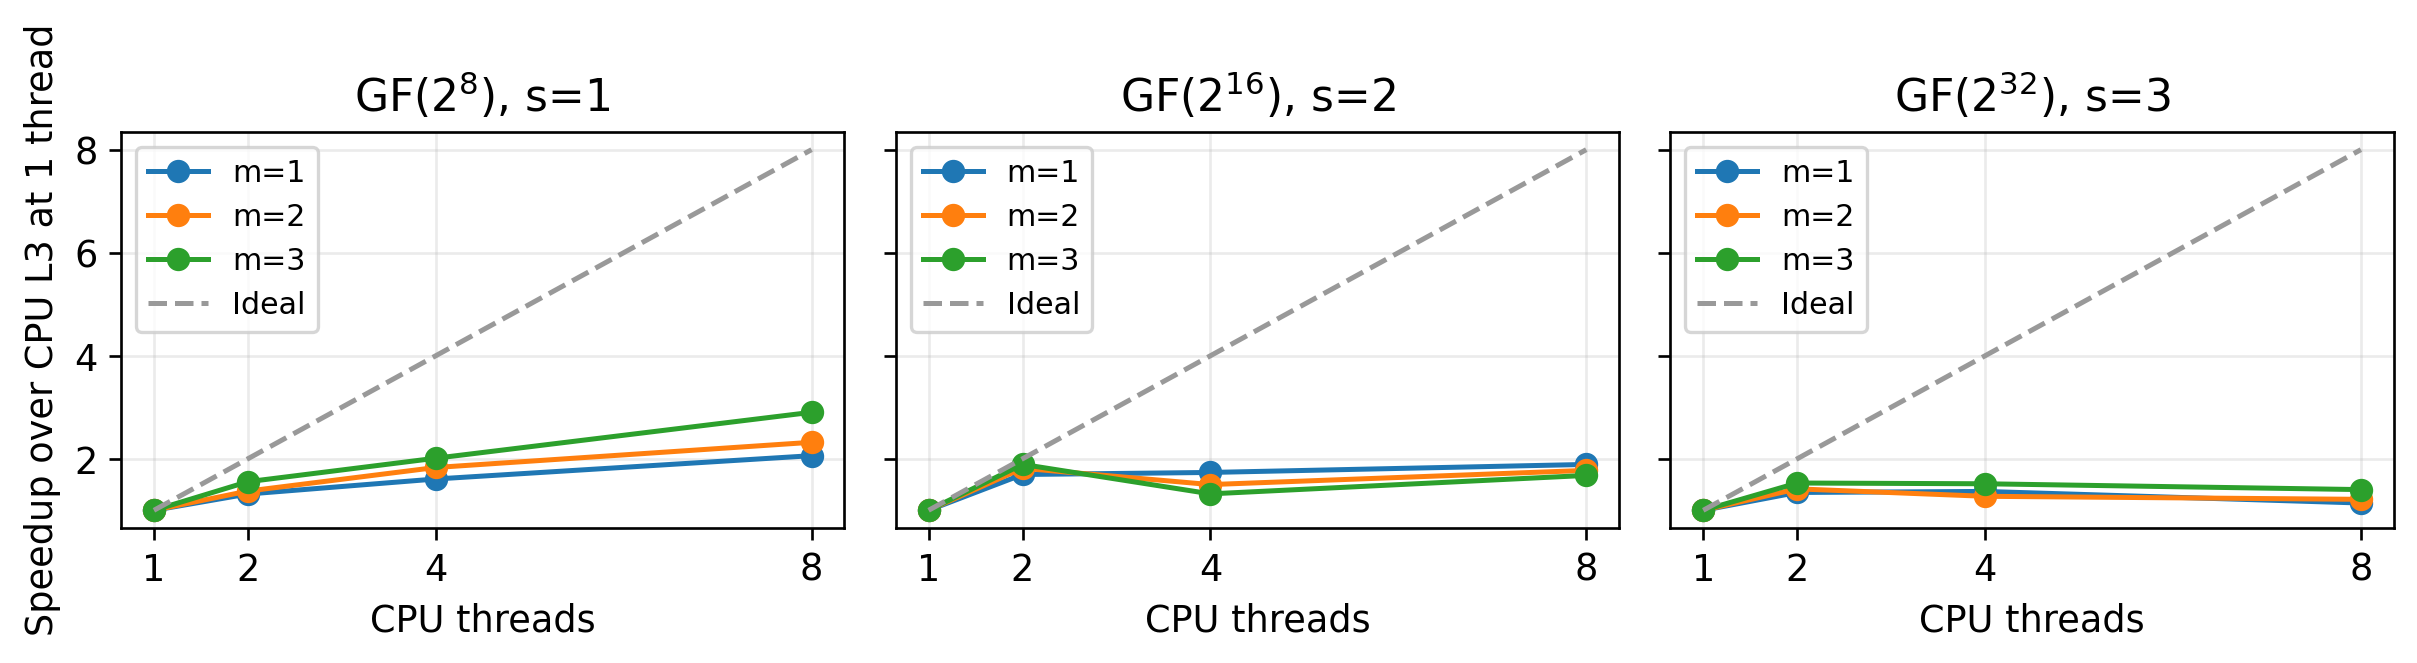
\includegraphics[width=0.90\textwidth]{../../results/milestone4/cpu_thread_scaling.png}
\caption{Final CPU thread scaling on nine 32 MiB workloads. Speedup is relative to the one-thread L3 median for the same workload; dashed lines denote ideal scaling.}
\label{fig:scaling}
\end{figure*}

\begin{figure*}[t]
\centering
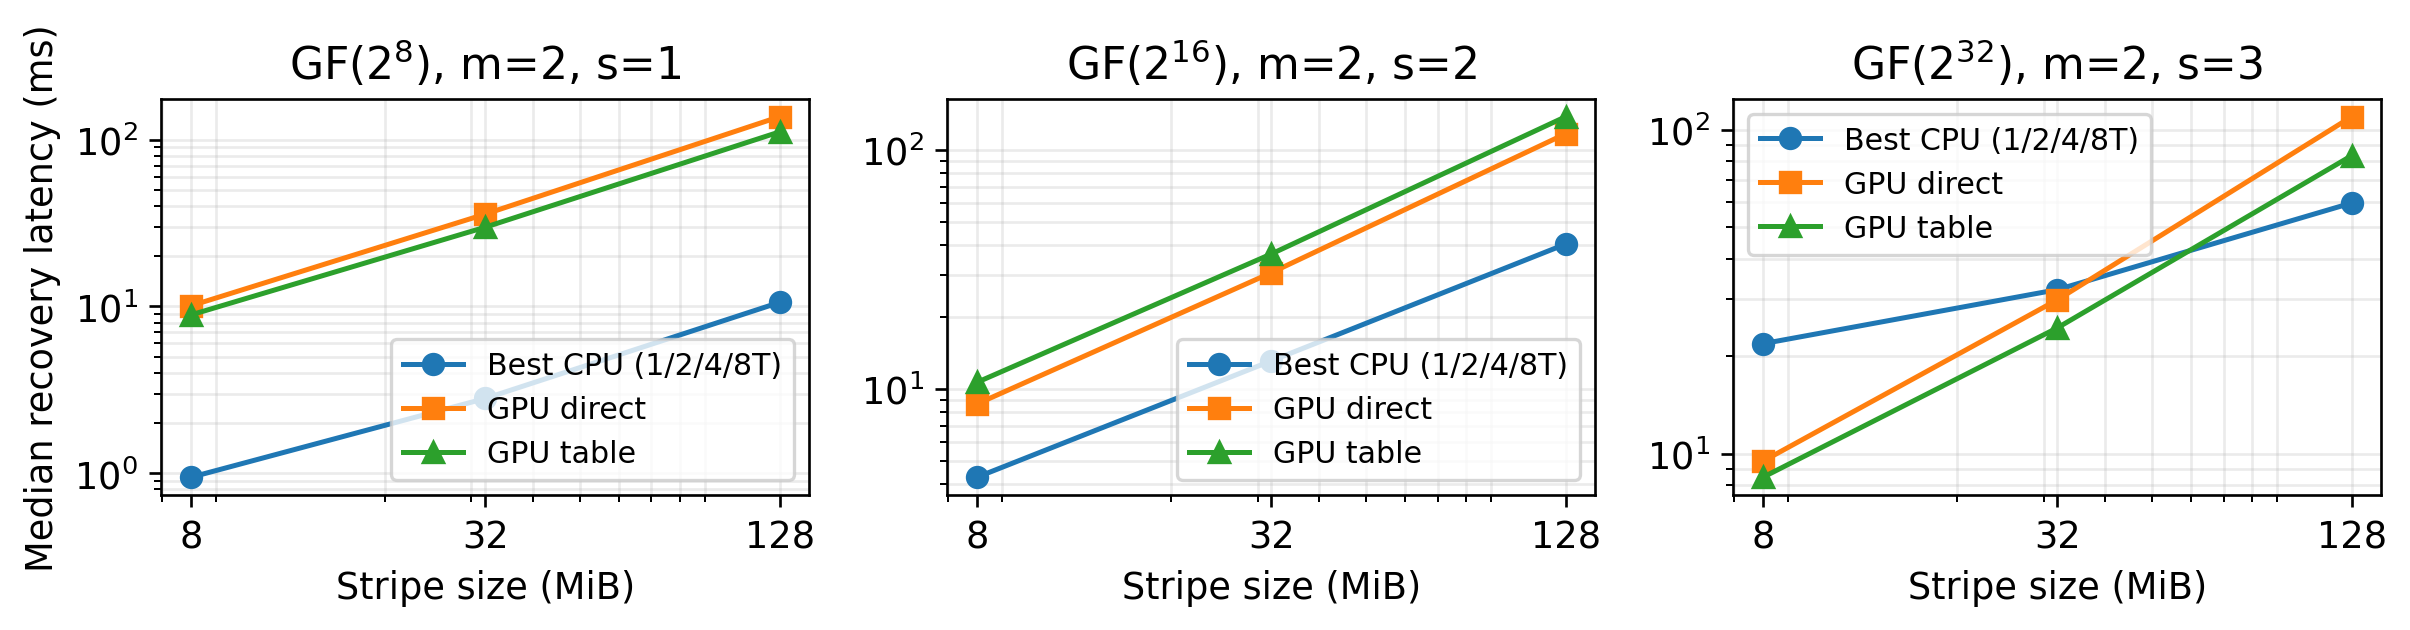
\includegraphics[width=0.90\textwidth]{../../results/milestone4/stripe_size_scaling.png}
\caption{Final end-to-end median latency versus stripe size at $m=2$. The CPU curve selects the lowest median among $T=1,2,4,8$ independently at each size. Both axes are logarithmic.}
\label{fig:sizes}
\end{figure*}

\subsection{Final CPU/GPU comparison}
Table~\ref{tab:final} reports final same-experiment medians. At 32 MiB, GPU table recovery beats the best tested CPU setting by 1.25$\times$--1.39$\times$ in the three GF($2^{32}$) cases, but is slower for every GF($2^8$) and GF($2^{16}$) case. GPU table is also slower than GPU direct for all GF($2^{16}$) cases. These are full-decoder comparisons: separately calibrated weights can change sequence selection and logical work, so they do not isolate table-kernel acceleration.

\begin{table*}[t]
\caption{Final 32 MiB end-to-end median recovery time in ms. CPU columns use L3 at the indicated thread count; GPU times include transfers and setup. Best $T$ minimizes the four CPU medians. Speedup is best CPU time divided by GPU table time.}
\label{tab:final}
\centering
\small
\setlength{\tabcolsep}{6pt}
\begin{tabular}{ccrrrrrrrr}
\hline
$m$ & $w$ & CPU 1T & CPU 2T & CPU 4T & CPU 8T & GPU direct & GPU table & Best $T$ & Speedup\\
\hline
1&8&4.089&3.108&2.544&1.985&22.702&21.131&8&0.09$\times$\\
1&16&16.617&9.803&9.578&8.791&21.619&27.699&8&0.32$\times$\\
1&32&34.327&25.499&25.124&30.079&22.640&20.169&4&1.25$\times$\\
2&8&6.496&4.730&3.548&2.800&35.804&29.888&8&0.09$\times$\\
2&16&23.796&13.101&15.871&13.407&30.613&36.665&2&0.36$\times$\\
2&32&45.473&32.116&35.755&37.495&29.877&24.476&2&1.31$\times$\\
3&8&8.198&5.272&4.076&2.825&45.572&37.817&8&0.07$\times$\\
3&16&31.103&16.444&23.577&18.545&36.630&40.537&2&0.41$\times$\\
3&32&60.862&39.790&40.172&43.417&34.436&28.644&2&1.39$\times$\\
\hline
\end{tabular}
\end{table*}

All final timed variants select partitioned recovery, though their selected sequences can differ. The best CPU setting is chosen from the same measured session; selecting the minimum of noisy medians may favor the CPU and is not a separate held-out tuning evaluation.

\section{GPU Advantage versus CPU Parallelism}
\label{sec:gpu-threads}
The comparison above selects the CPU's best tested thread count. This section examines how the GPU's advantage changes as each additional CPU thread is added, and where it crosses parity.

\begin{figure*}[t]
\centering
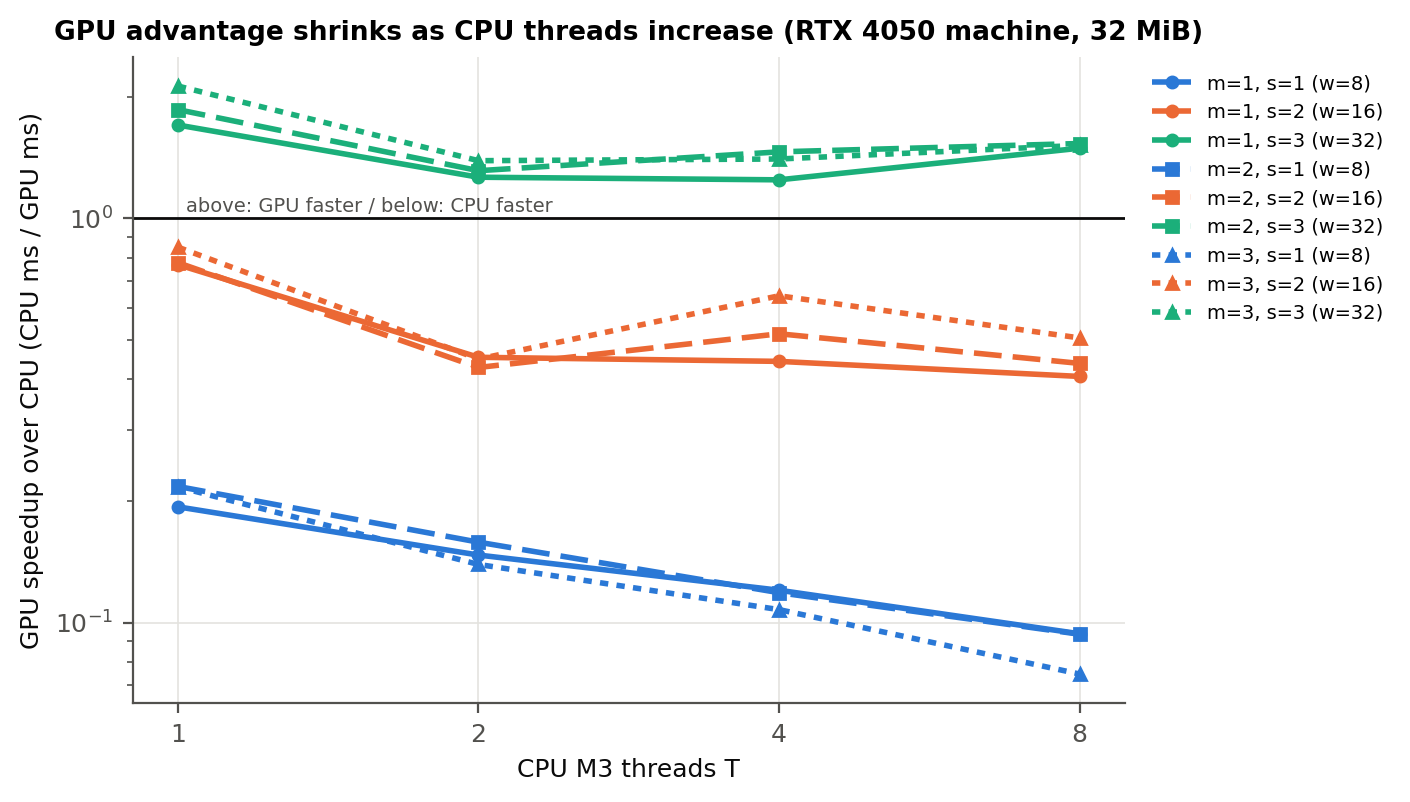
\includegraphics[width=0.80\textwidth]{../../results/evaluation/figures/gpu_speedup_vs_cpu_threads.png}
\caption{GPU speedup over CPU L3 (gPPM) as CPU threads increase, Core Ultra 9 185H + RTX 4050, 32 MiB, same session. Values above one mean the GPU is faster. The GPU uses the faster of its two kernels. Both axes are logarithmic.}
\label{fig:gpu-threads}
\end{figure*}

\subsection{Same-machine measurements}
Fig.~\ref{fig:gpu-threads} plots the ratio of CPU to GPU median time from the 900-trial session. Three regimes appear and are set by the field:
\begin{itemize}
\item \textbf{GF($2^8$):} the GPU is 4.5$\times$--14$\times$ slower. Its disadvantage grows with every thread, from 0.19--0.22 at $T=1$ to 0.07--0.09 at $T=8$.
\item \textbf{GF($2^{16}$):} the GPU is slower at every thread count, at 0.41--0.85.
\item \textbf{GF($2^{32}$):} the GPU is faster at every tested thread count, but its lead shrinks from 1.70$\times$--2.12$\times$ at $T=1$ to 1.25$\times$--1.40$\times$ at $T=2$ or 4. It then widens again at $T=8$ (1.49$\times$--1.53$\times$), because CPU scaling reverses.
\end{itemize}
Table~\ref{tab:gpu-ratio} lists the ratios. Stripe size moves the crossover. For $(m,s)=(2,3)$, the ratio at $T=1,2,4,8$ is 3.10, 2.58, 3.08, 2.82 at 8 MiB, but 1.78, 1.05, 0.71, 0.94 at 128 MiB. At 128 MiB the CPU therefore \emph{overtakes the GPU at $T\approx2.3$}, interpolated between two and four threads. This is the one same-machine thread-count crossover in the data. With the best CPU thread count at each size, log-interpolation puts the size crossover near 66 MiB.

\begin{table}[t]
\caption{GPU speedup over CPU L3 at each CPU thread count (CPU median / best-GPU median), Core Ultra 9 + RTX 4050, 32 MiB unless noted. Above one: GPU faster.}
\label{tab:gpu-ratio}
\centering
\footnotesize
\setlength{\tabcolsep}{4pt}
\begin{tabular}{cc rrrr l}
\hline
$m$ & $w$ & $T{=}1$ & $T{=}2$ & $T{=}4$ & $T{=}8$ & Faster\\
\hline
1&8&0.19&0.15&0.12&0.09&CPU at all $T$\\
2&8&0.22&0.16&0.12&0.09&CPU at all $T$\\
3&8&0.22&0.14&0.11&0.07&CPU at all $T$\\
1&16&0.77&0.45&0.44&0.41&CPU at all $T$\\
2&16&0.78&0.43&0.52&0.44&CPU at all $T$\\
3&16&0.85&0.45&0.64&0.51&CPU at all $T$\\
1&32&1.70&1.26&1.25&1.49&GPU at all $T$\\
2&32&1.86&1.31&1.46&1.53&GPU at all $T$\\
3&32&2.12&1.39&1.40&1.52&GPU at all $T$\\
\hline
\multicolumn{2}{l}{$(2,32)$, 8 MiB}&3.10&2.58&3.08&2.82&GPU at all $T$\\
\multicolumn{2}{l}{$(2,32)$, 128 MiB}&1.78&1.05&0.71&0.94&CPU from $T{\approx}2.3$\\
\hline
\end{tabular}
\end{table}

\subsection{Projected fine-grained crossover}
The GPU session tested only $T=1,2,4,8$. To locate the GF($2^{32}$) crossover more precisely, we measured CPU L3 at every $T=1$--16 on a second machine (Section~\ref{sec:ext-platform}). Each GPU time was scaled by the ratio of single-thread L3 medians between the two CPUs. That factor is 0.91--0.95 for GF($2^{32}$), so the scaling cancels single-core speed differences but not memory-system differences. The scaled ratios are a projection, not a co-located measurement.

Fig.~\ref{fig:gpu-proj} shows the result. With operating-system thread placement, the GPU stays ahead at every $T$, with a minimum lead of 1.13$\times$--1.20$\times$ at $T=2$--3. With threads bound one per performance core, the ratio falls to 1.03--1.14 at $T=3$ and \emph{crosses parity between $T=3$ and 4}: interpolated at $T=3.5$, 3.6, and 3.8 for $m=1,2,3$. At $T=4$ it reaches 0.95--0.97. The margin is within run-to-run variation, so it amounts to parity rather than a clear CPU win. At $T=5$, when the fifth thread lands on an efficiency core, the GPU lead jumps back to 2.53$\times$--2.93$\times$. Hyper-Threading siblings reduce it only to 1.56$\times$--1.66$\times$ by $T=12$.

\begin{figure}[t]
\centering
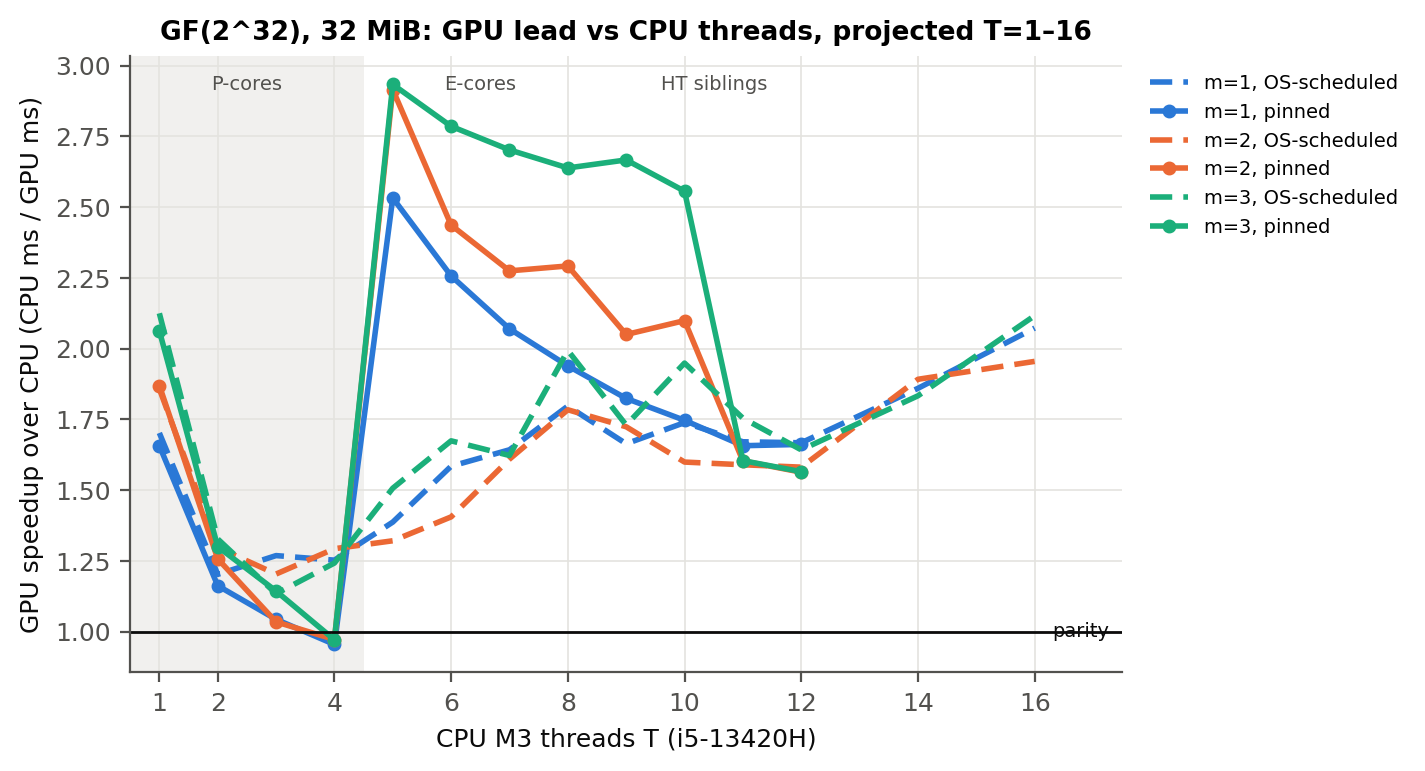
\includegraphics[width=\columnwidth]{../../results/evaluation/figures/gpu_speedup_vs_cpu_threads_projected.png}
\caption{Projected GPU speedup over CPU L3 for GF($2^{32}$) at 32 MiB, $T=1$--16 on the i5-13420H. Solid: threads bound to performance cores, then efficiency cores, then Hyper-Threading siblings. Dashed: OS scheduling.}
\label{fig:gpu-proj}
\end{figure}

Fig.~\ref{fig:combined} places M2 (scalar PPM), M3 (L3), and the GPU on a common scale, using speedup over the scalar sequential decoder. The GPU beats M2 at every thread count in every field. M2 never drops below 30 ms at 32 MiB, because its serial remainder limits it (Section~\ref{sec:taper}). Against M3, the GPU wins only in GF($2^{32}$).

\begin{figure*}[t]
\centering
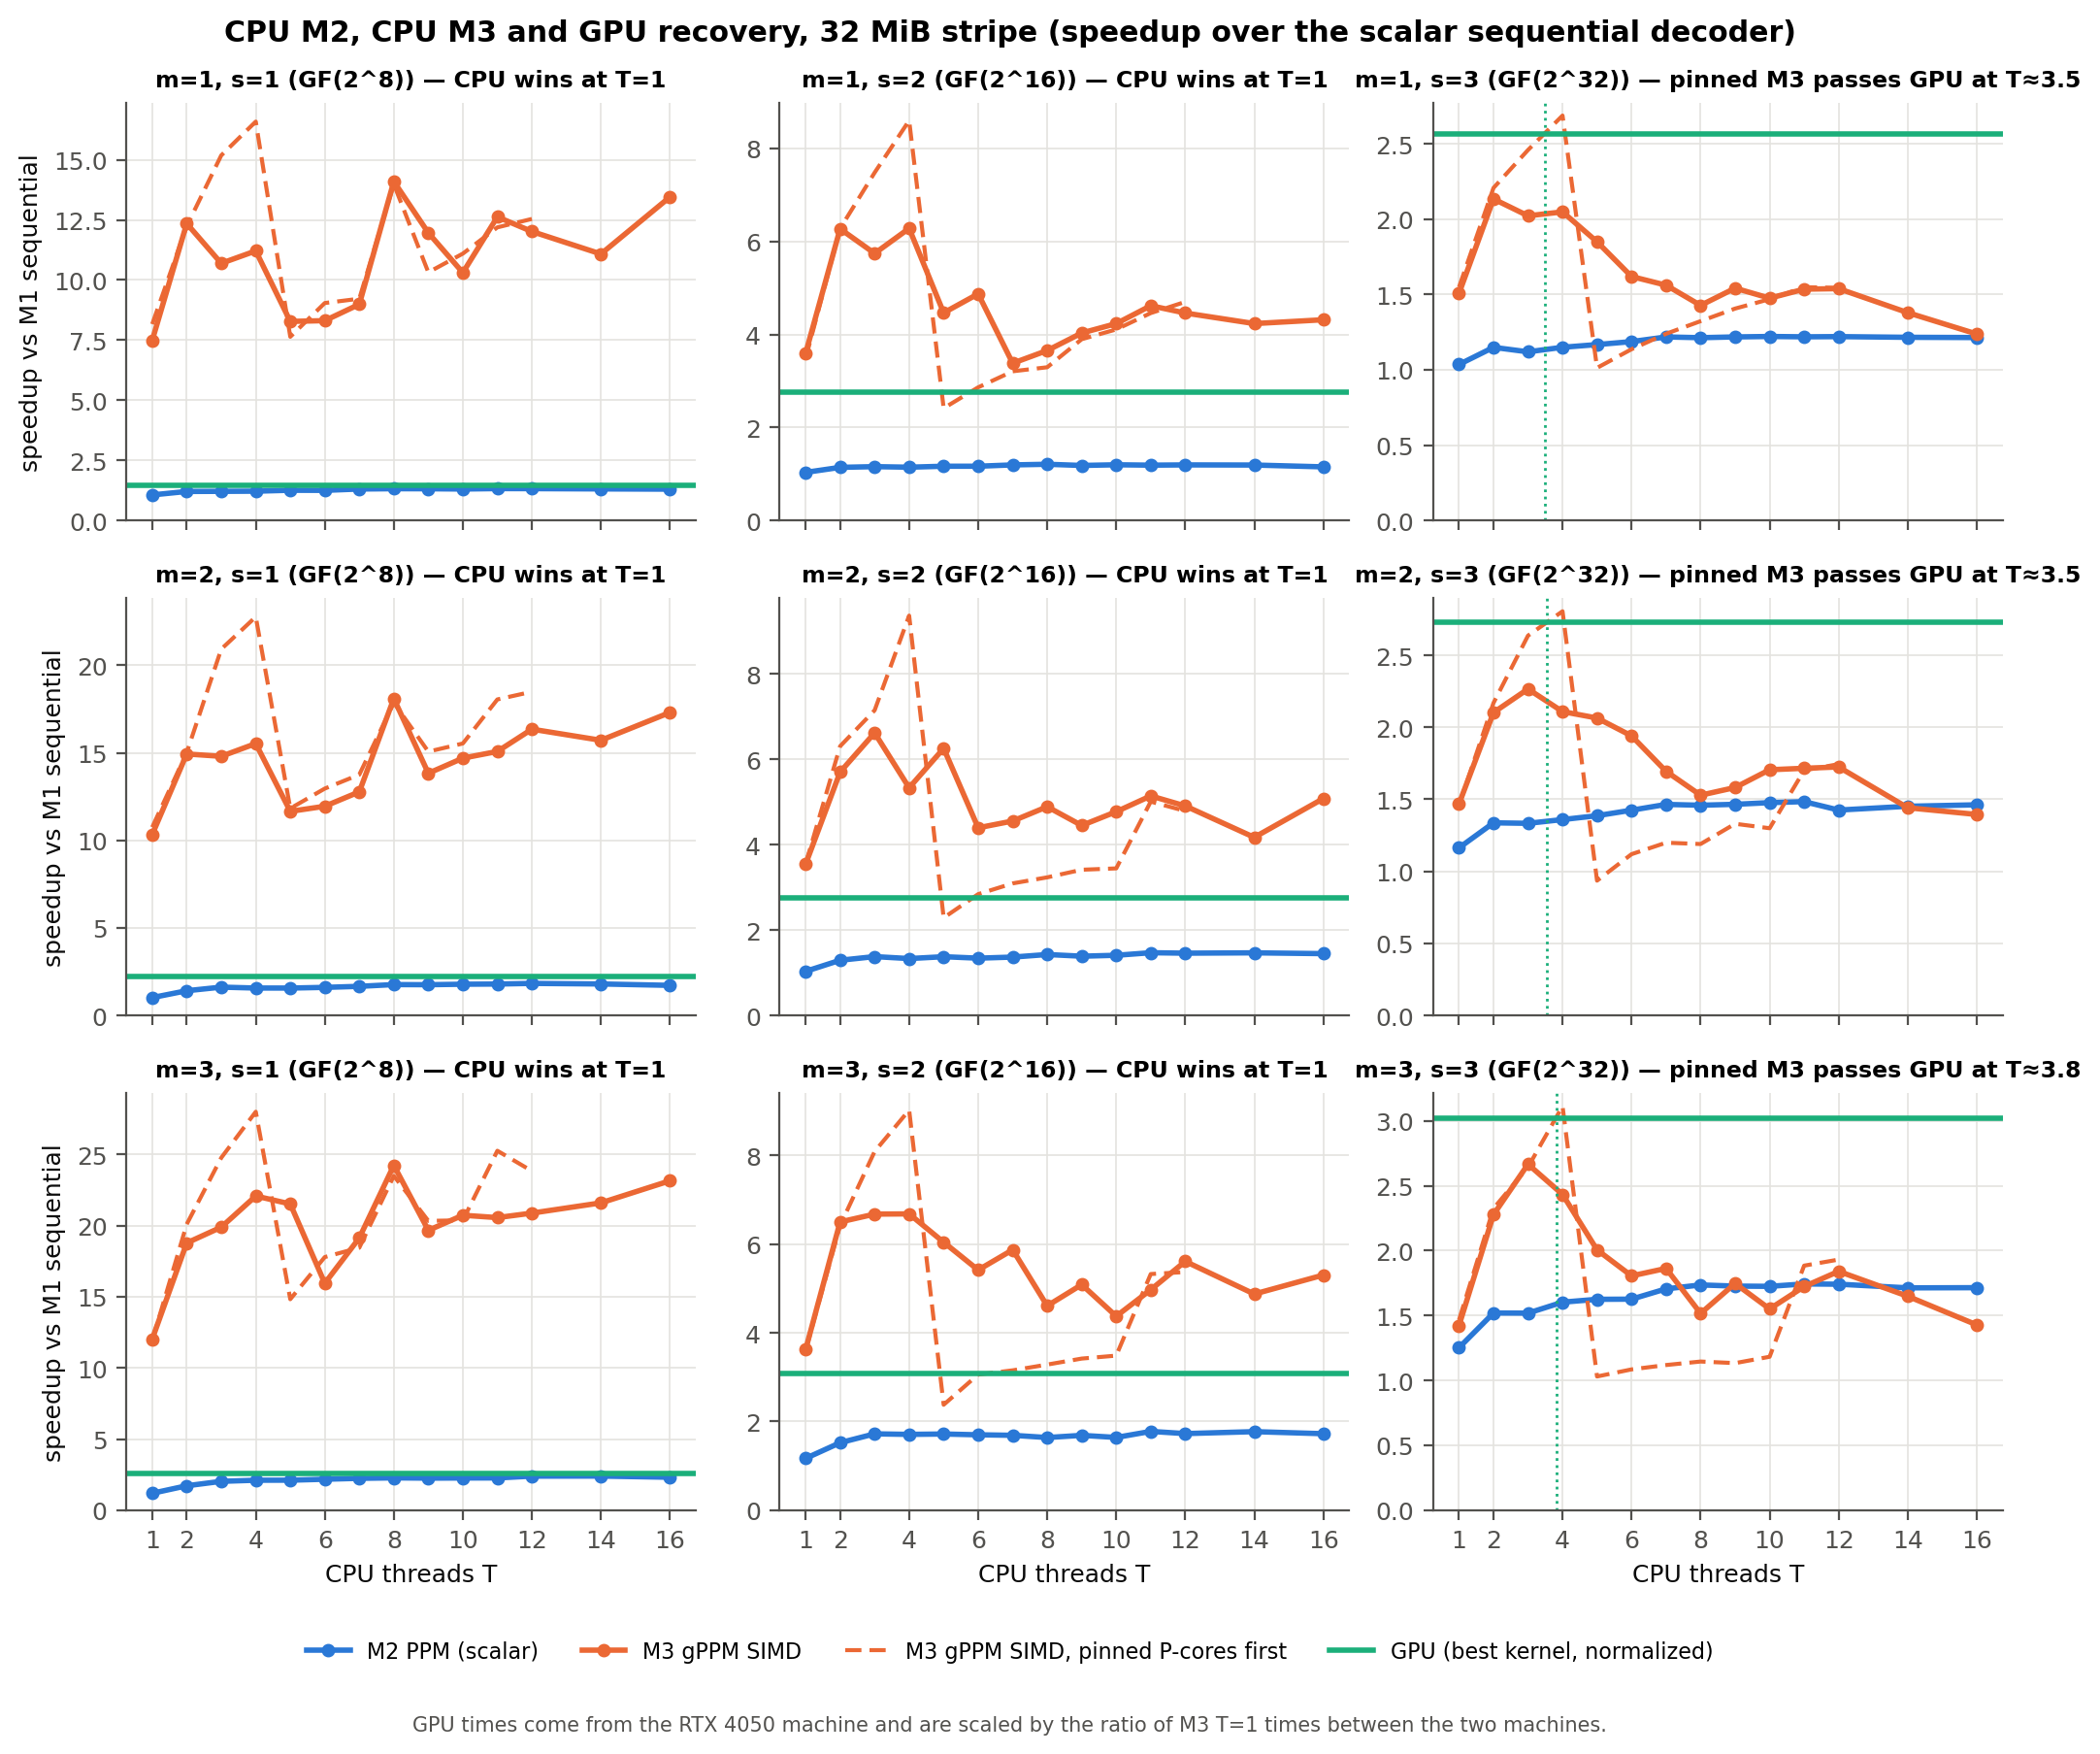
\includegraphics[width=0.92\textwidth]{../../results/evaluation/figures/combined_m2_m3_gpu_speedup.png}
\caption{M2, M3 (OS-scheduled and pinned), and GPU recovery on a common scale: speedup over the scalar sequential decoder, 32 MiB, $n=r=16$. CPU curves are from the i5-13420H. The GPU line is the RTX 4050 time scaled by the single-thread L3 ratio between the two machines. Panel titles give the crossover.}
\label{fig:combined}
\end{figure*}

\section{Extended CPU Evaluation}
\subsection{Platform and method}
\label{sec:ext-platform}
The extended runs use an Intel Core i5-13420H with 4 performance cores with Hyper-Threading (logical CPUs 0--7) and 4 efficiency cores (CPUs 8--11), running in the ``balanced'' power profile. One benchmark driver is compiled against each milestone decoder:
\begin{itemize}
\item M1: scalar sequential recovery.
\item M2: fixed-sequence PPM with a serial remainder.
\item M2+SIMD: M2's schedule linked with M3's SIMD arithmetic, which is the original paper's PPM.
\item M3: scalar and SIMD builds, with serial or parallel remainder.
\end{itemize}
OpenMP dynamic teams are disabled.

Each configuration runs one warm-up, then 10 trials for thread scaling or 5--7 for parameter grids. Variants are shuffled within every round. A placement control binds threads 1--4 to performance cores, 5--8 to efficiency cores, and 9--12 to Hyper-Threading siblings (\texttt{OMP\_PLACES}, \texttt{OMP\_PROC\_BIND=close}). All 23,028 trials match the encoded stripe and have zero syndrome.

\subsection{Where speedup tapers off}
\label{sec:taper}
Fig.~\ref{fig:pinned} and Table~\ref{tab:taper} summarize scaling over $T=1$--16.
\begin{itemize}
\item \textbf{M2} is limited by its serial remainder. Fitting $S(T)=1/(f+(1-f)/T)$ for $T\le8$ gives serial fractions $f=0.44$--0.85, which bounds speedup at 1.2$\times$--2.3$\times$. The last thread count that still gains at least 5\% is $T=2$--4.
\item \textbf{SIMD aggravates the limit.} It accelerates only the parallel groups, so M2+SIMD reaches 1.00$\times$--1.48$\times$ and does not scale at all for $(m,s)=(1,3)$.
\item \textbf{M3 parallelizes the remainder.} Under OS scheduling it peaks at $T=8$ for GF($2^8$) and at $T=2$--4 for wider fields, with jagged curves.
\item \textbf{Placement removes the ambiguity.} With bound threads, M3 peaks at \emph{exactly $T=4$ in all nine configurations}, reaching 1.74$\times$--2.64$\times$. At $T=5$ it loses 47--76\% of that speed (0.64$\times$--1.24$\times$ its $T=1$ speed). Static scheduling waits for the slowest worker, which is now an efficiency core.
\item \textbf{Oversubscription.} At $T=16$, GF($2^{32}$) falls back to 0.82$\times$--1.00$\times$ of its $T=1$ speed.
\end{itemize}
Parallel speedup on this CPU therefore wears off after the fourth thread, the number of performance cores. The original paper reports the same rule, with maximum improvement at $T=$ core count.

\begin{figure*}[t]
\centering
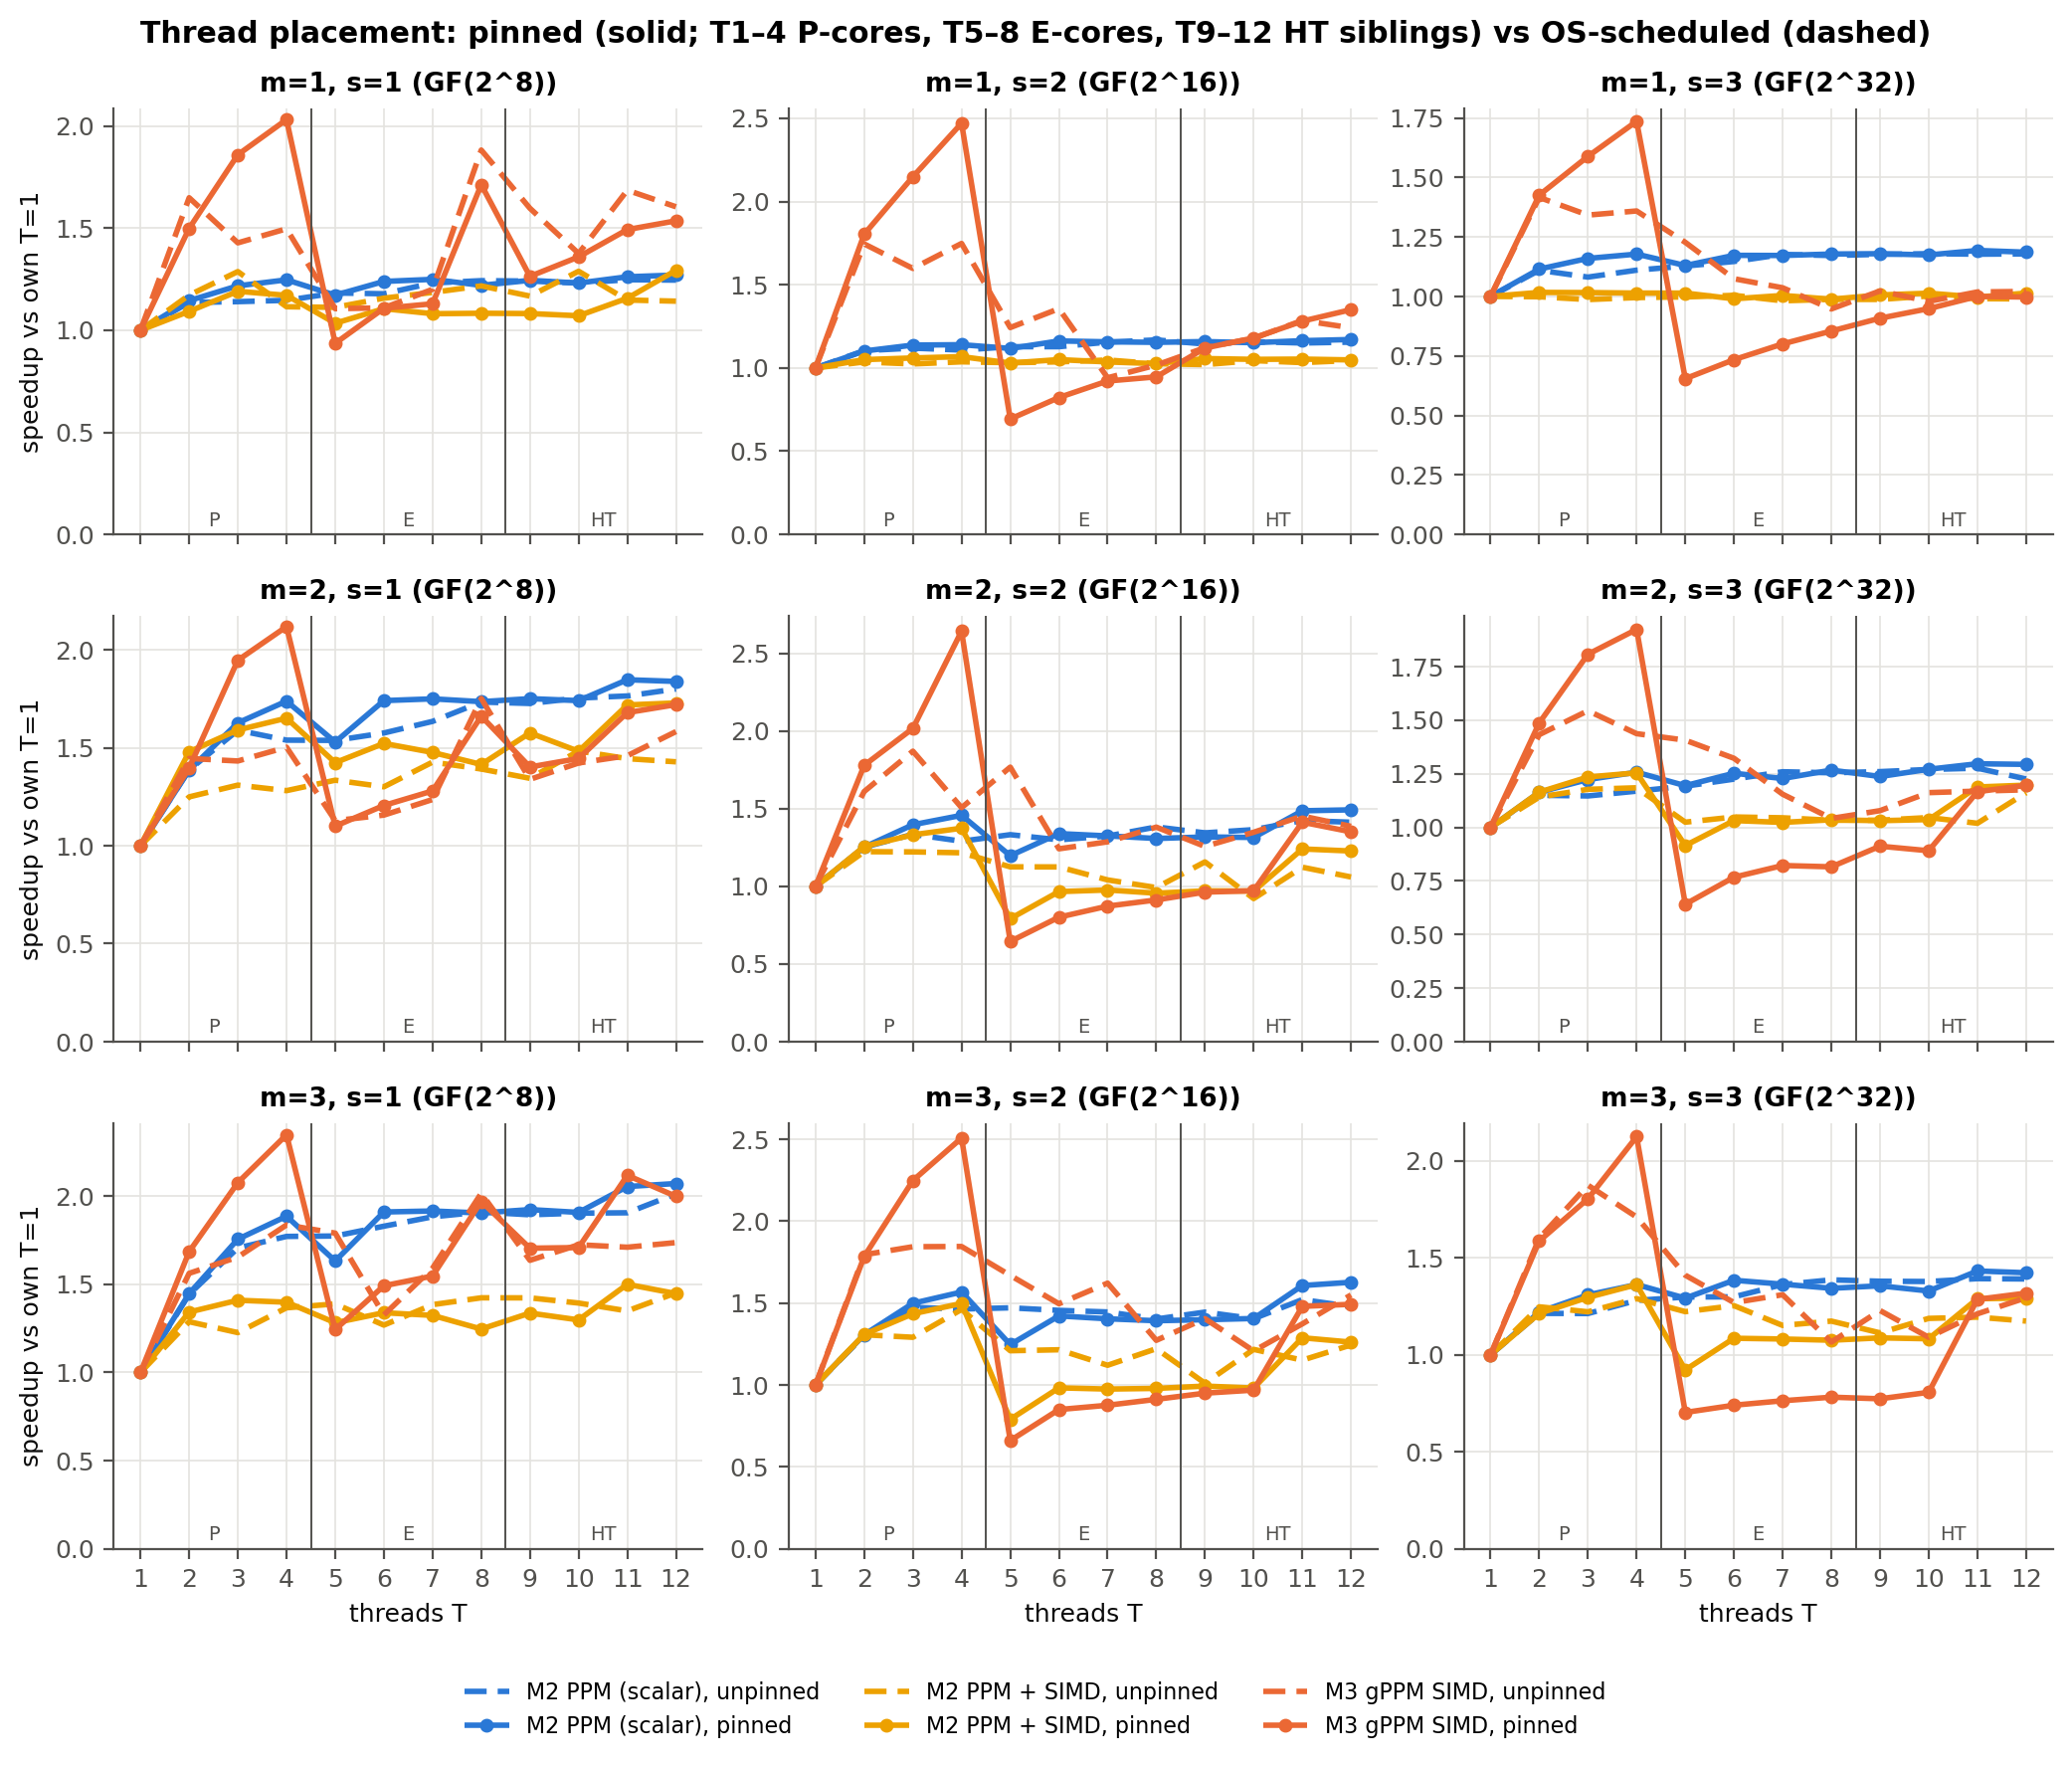
\includegraphics[width=0.90\textwidth]{../../results/evaluation/figures/scaling_pinned_vs_unpinned.png}
\caption{Speedup over each implementation's own $T=1$ median, i5-13420H, 32 MiB. Solid: bound placement (P = performance cores, E = efficiency cores, HT = Hyper-Threading siblings). Dashed: OS scheduling.}
\label{fig:pinned}
\end{figure*}

\begin{table}[t]
\caption{Taper metrics over nine $(m,s)$ configurations, 32 MiB. ``Knee'' is the last $T$ whose increment gains $\ge$5\%. $f$ is the fitted Amdahl serial fraction ($T\le8$).}
\label{tab:taper}
\centering
\footnotesize
\setlength{\tabcolsep}{3pt}
\begin{tabular}{l rrrr}
\hline
Implementation & Peak $S$ & Peak $T$ & Knee $T$ & $f$\\
\hline
M2 (scalar) & 1.17--2.02 & 8--14 & 2--4$^\dagger$ & 0.44--0.85\\
M2+SIMD & 1.00--1.48 & 2--12 & 1--4$^\dagger$ & 0.67--1.00\\
M3, OS-scheduled & 1.42--2.02 & 2--8 & 2--8 & 0.49--0.83\\
M3, bound & 1.74--2.64 & \textbf{4} & \textbf{4} & --\\
\hline
\multicolumn{5}{l}{$^\dagger$GF($2^8$) with $m\ge2$ creeps upward to $T=7$--12.}\\
\end{tabular}
\end{table}

\subsection{Ablation}
Table~\ref{tab:ablation} adds techniques one at a time, reported as speedup over M1. Partitioning alone gives 1.10$\times$. SIMD is the largest single step, reaching 3.63$\times$ geometric mean and 12.2$\times$ for $(3,1)$. Cost selection raises this to 3.75$\times$. Four threads on the independent groups alone give 4.29$\times$, and parallelizing the remainder gives \textbf{5.93$\times$}. Going on to eight threads lowers the result to 4.92$\times$.

Removing one technique at a time from M3 at $T=8$ slows recovery by:
\begin{itemize}
\item SIMD: 1.77$\times$.
\item Partitioning: 1.46$\times$.
\item Multithreading: 1.32$\times$.
\item Parallel remainder: 1.21$\times$.
\item Sequence selection: 1.18$\times$.
\end{itemize}
For GF($2^{32}$) only, removing SIMD is \emph{faster} at $T=8$ (0.68$\times$--0.77$\times$ the time). The AVX2 kernel rebuilds coefficient tables per region (Section~\ref{sec:profile}), and that cost scales poorly onto efficiency cores. The full factorial over arithmetic, sequence, remainder, and $T\in\{1,2,4,8,12\}$ is in the repository.

\begin{table}[t]
\caption{Cumulative layer ablation: geometric-mean speedup over M1 for nine $(m,s)$, i5-13420H, 32 MiB, $n=r=16$. Each row adds one technique.}
\label{tab:ablation}
\centering
\footnotesize
\setlength{\tabcolsep}{3pt}
\begin{tabular}{l rr}
\hline
Layer & Geomean & Range\\
\hline
M1 sequential scalar & 1.00$\times$ & --\\
+ PPM partition, fixed sequence ($T{=}1$) & 1.10$\times$ & 1.01--1.25\\
+ SIMD region arithmetic & 3.63$\times$ & 1.38--12.22\\
+ gPPM cost-selected sequence & 3.75$\times$ & 1.45--13.31\\
+ 4 threads, groups only & 4.29$\times$ & 1.53--16.64\\
+ parallel remainder ($T{=}4$) & \textbf{5.93$\times$} & 2.05--22.08\\
+ 8 threads & 4.92$\times$ & 1.43--24.24\\
\hline
\end{tabular}
\end{table}

\subsection{Code parameters}
We measured 306 feasible codes with $n,r\in\{4,8,\dots,24\}$ and $m,s\in\{1,2,3\}$ at $T=4$, comparing M2+SIMD against sequential SIMD recovery. The mean PPM improvement varies with each parameter:
\begin{itemize}
\item It falls with $n$: +77\%, 43\%, 29\%, 27\%, 25\%, 23\% for $n=4$--24.
\item It rises with $r$: +25\% to +41\%.
\item It rises with $m$: +10\%, 36\%, 63\%.
\item It falls with $s$: +62\%, 26\%, 14\%.
\end{itemize}
These are the directions the original paper reports. Field width is fixed by the published coefficients for each $(n,m,s,r)$, so it cannot be varied independently. Grouped by field, mean improvement is +22\% to +88\% for GF($2^8$), 0\% to +51\% for GF($2^{16}$), and $-7$\% to +35\% for GF($2^{32}$), increasing with $m$.

Stripe size and failure rows also matter. At 1--4 MiB, PPM is slower than SD in five of nine configurations, and from 64 MiB it is faster in all nine. Spreading sector failures over $z=2$ or 3 rows leaves the $T=4$ M3 gain between +28\% and +154\%.

\subsection{Reproducing the original evaluation}
Fig.~\ref{fig:repro} reproduces the original paper's Figs.~10, 11, 13 and 17 with our decoders, and Table~\ref{tab:repro} compares headline numbers. Our maximum PPM improvement (+259\%) exceeds the published 210.81\%. Our mean (+35\%) is lower because, unlike the paper, we report configurations where PPM is slower (minimum $-18.7$\%).

For gPPM over PPM we compare at $T=1$. At higher $T$, M3's parallel remainder, which M2 lacks, would be credited to sequence selection. On that basis, 27\% of configurations improve by more than 5\%, close to the paper's ``nearly 1/3'', with a maximum of +63.7\%.

Figs.~12 and 14--16 are not reproduced. Fig.~12 compares three server CPUs, and Figs.~14--16 evaluate LRC, RS, and GRS codes, which this project does not implement.

\begin{table}[t]
\caption{Original paper (E5-2603, $T\le4$) vs.\ this reproduction (i5-13420H). Improvement is PPM/SD$-1$, both with SIMD.}
\label{tab:repro}
\centering
\footnotesize
\setlength{\tabcolsep}{3pt}
\begin{tabular}{l rr}
\hline
Metric & Paper & Ours\\
\hline
Max PPM improvement & 210.81\% & 259.0\%\\
Mean PPM improvement ($T{=}4$) & 61.09\% & 35.1\%\\
Mean improvement at $T{=}2$ & 46.29\% & 28.8\%\\
Max gPPM over PPM & 102.41\% & 63.7\%\\
Configs where gPPM wins & $\approx$1/3 & 27\%\\
\hline
\end{tabular}
\end{table}

\begin{figure*}[t]
\centering
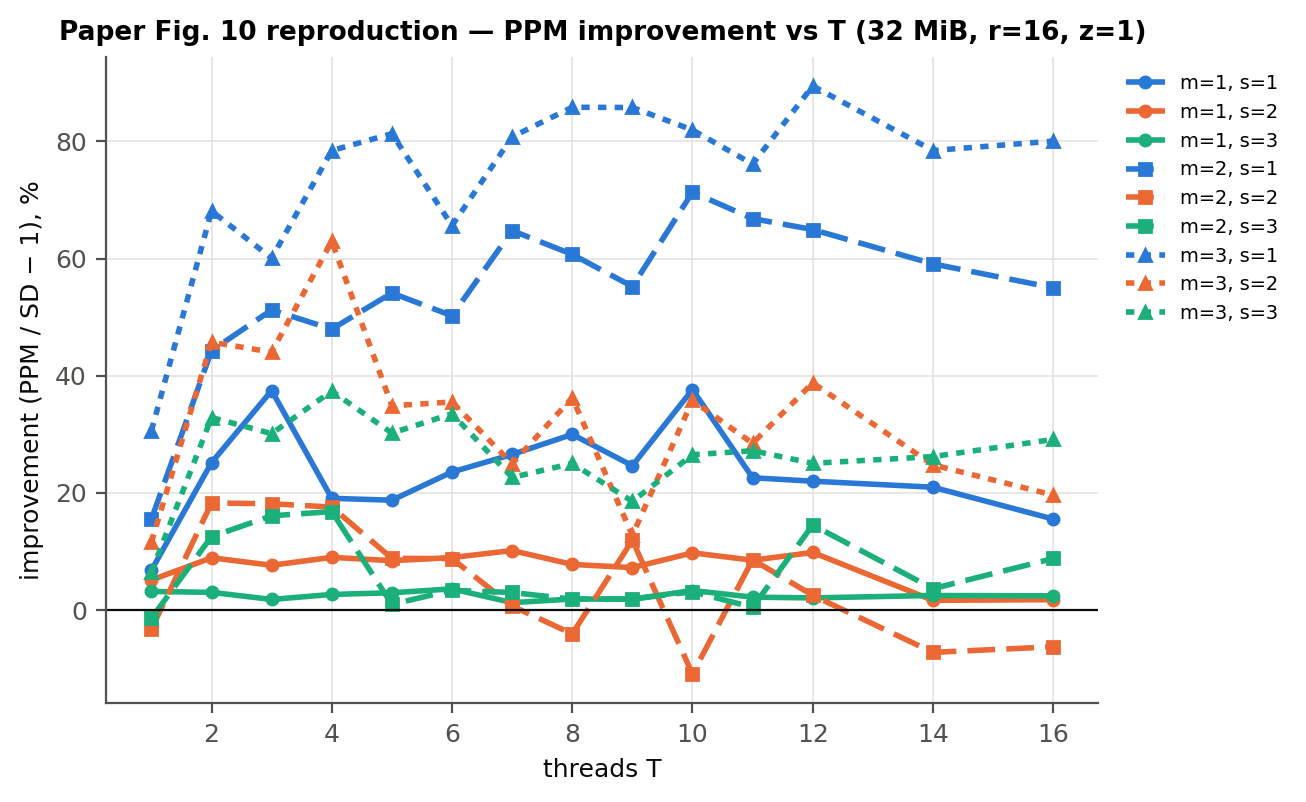
\includegraphics[width=0.49\textwidth]{../../results/evaluation/figures/paper_fig10_improvement_vs_threads.png}\hfill
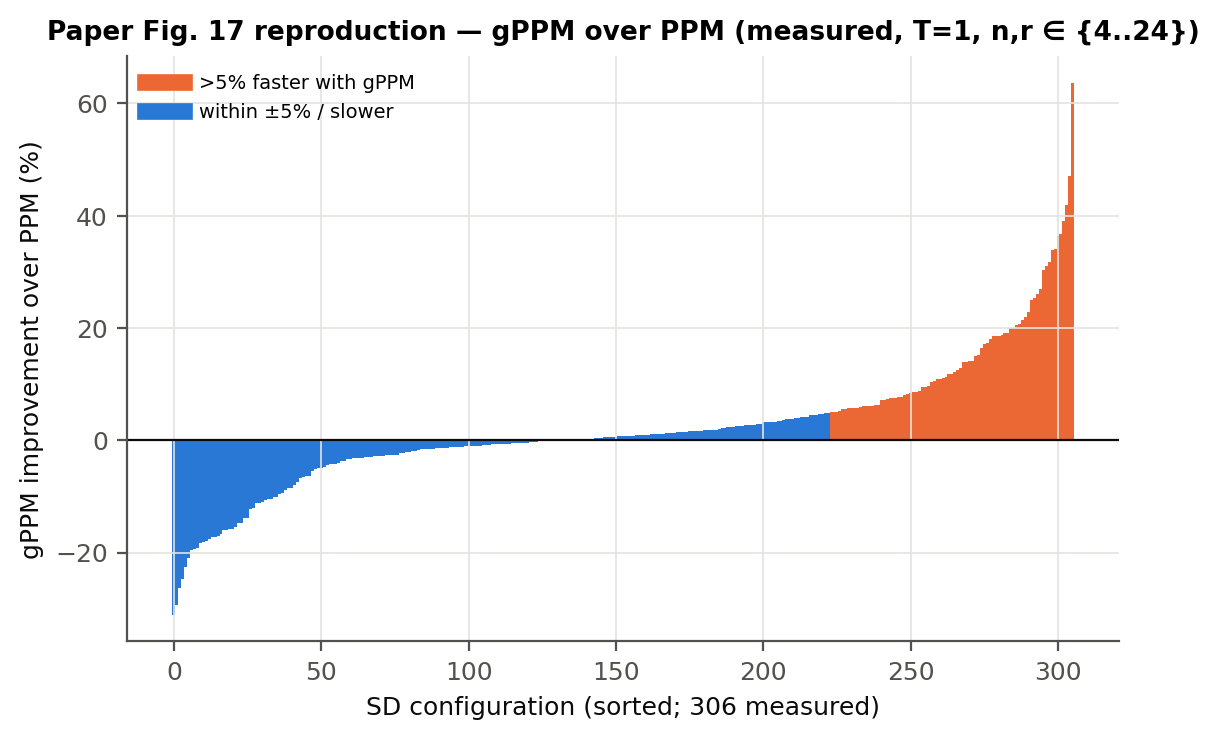
\includegraphics[width=0.49\textwidth]{../../results/evaluation/figures/paper_fig17_gppm_over_ppm_measured.png}\\[4pt]
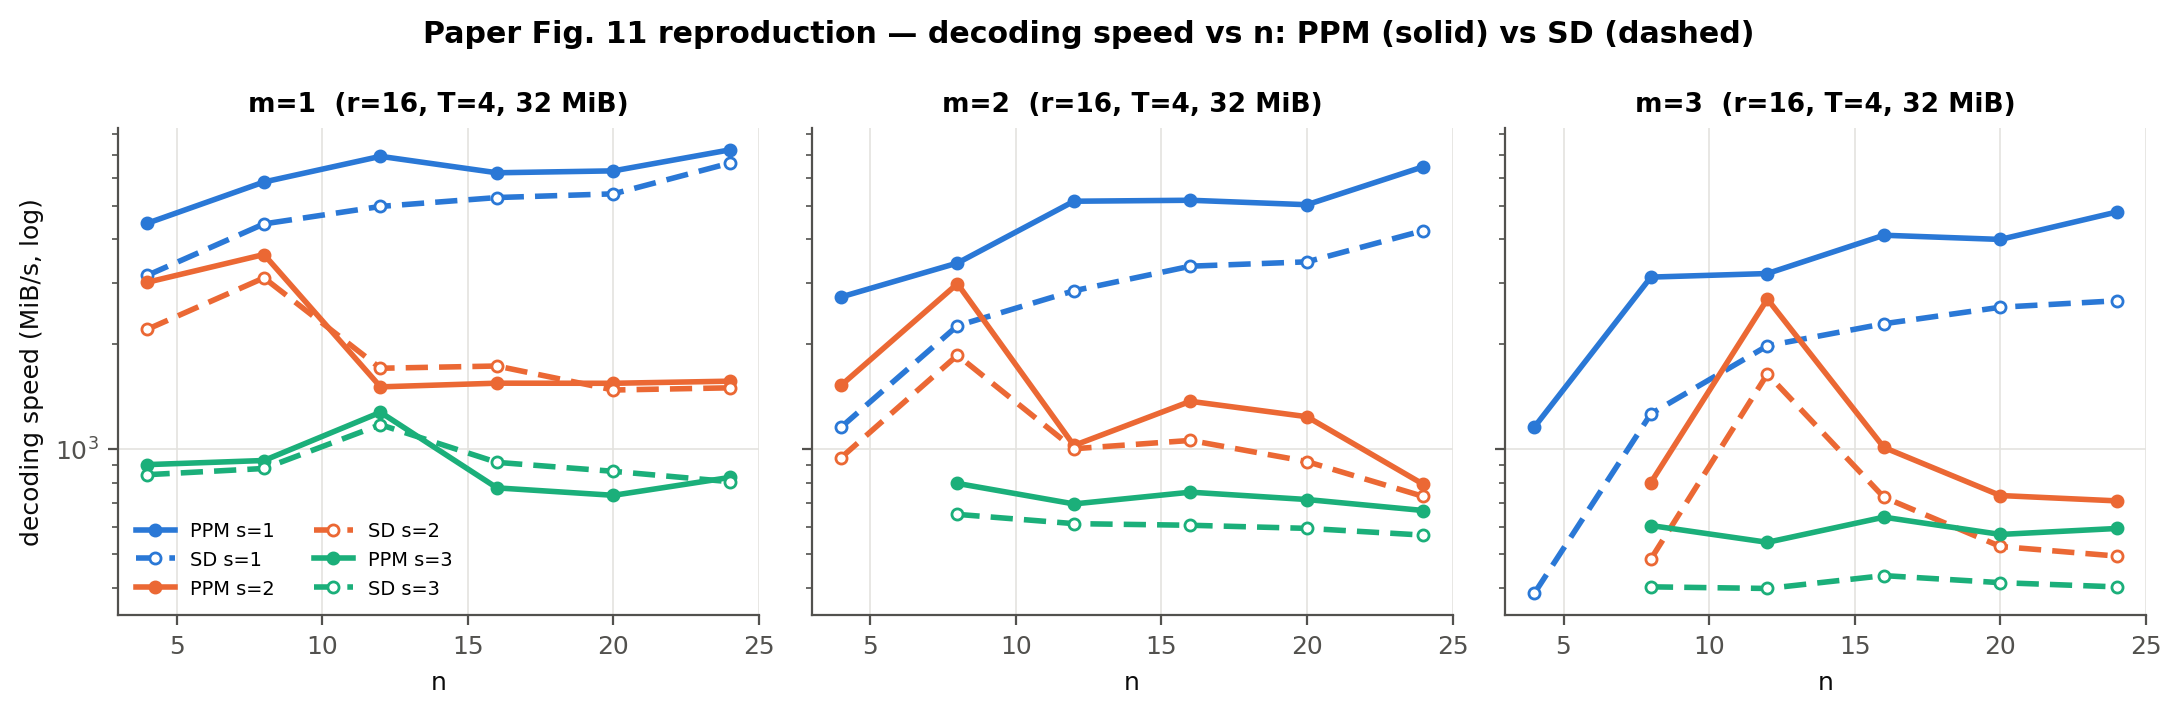
\includegraphics[width=0.98\textwidth]{../../results/evaluation/figures/paper_fig11_speed_vs_n.png}\\[4pt]
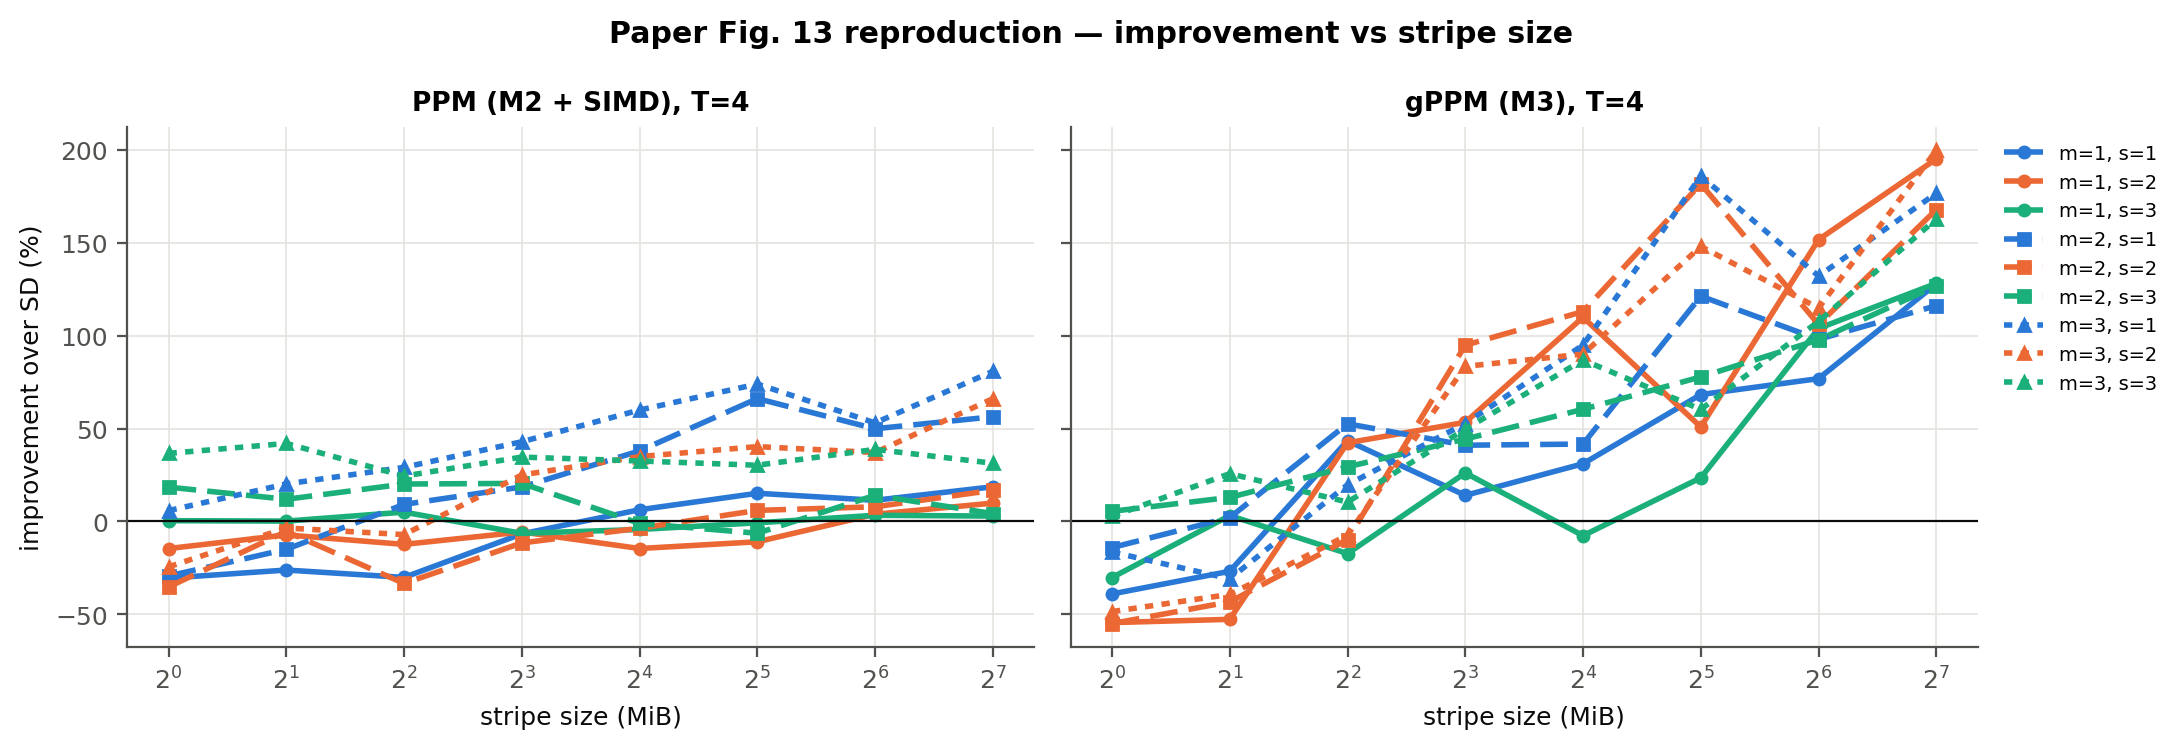
\includegraphics[width=0.98\textwidth]{../../results/evaluation/figures/paper_fig13_improvement_vs_stripe.png}
\caption{Reproductions of the original paper's evaluation on the i5-13420H, 32 MiB unless varied. Top left: improvement vs.\ $T$ (Fig.~10). Top right: gPPM over PPM at $T=1$ over 306 codes (Fig.~17). Middle: decoding speed vs.\ $n$ at $r=16$, $T=4$ (Fig.~11). Bottom: improvement vs.\ stripe size (Fig.~13).}
\label{fig:repro}
\end{figure*}

\section{Profiling and Bottleneck Analysis}
\subsection{CPU instruction profile}
\label{sec:profile}
Table~\ref{tab:cpu-profile} reports self instruction counts for one recovery per field. Region multiply-XOR and XOR functions account for 89.7\% and 93.4\% of instructions in the GF($2^8$) and GF($2^{16}$) profiles, respectively. In GF($2^{32}$), the scalar field-multiply routine alone accounts for 58.2\%; the call tree attributes 57.2 percentage points to calls from the AVX2 region kernel. That kernel constructs four 256-entry coefficient tables on each region operation before its gather loop. Reusing coefficient tables is therefore a concrete optimization candidate. Callgrind counts instructions under emulation, not native cycles or elapsed time; this single-thread profile does not explain all multithread scaling losses.

\begin{table}[t]
\caption{Recovery-only CPU Callgrind profile: $m=2$, 32 MiB, one thread. Self costs exclude callees; region includes multiply-XOR and XOR functions.}
\label{tab:cpu-profile}
\centering
\footnotesize
\begin{tabular}{rrrr}
\hline
$w$ & Instructions (million) & Region self & GF32 multiply self\\
\hline
8&100.9&89.7\%&0.0\%\\
16&161.7&93.4\%&0.0\%\\
32&359.2&38.4\%&58.2\%\\
\hline
\end{tabular}
\end{table}

\subsection{GPU trace and bottlenecks}
Table~\ref{tab:gpu-profile} summarizes separate recovery-only traces. In the GF($2^{32}$) table trace, kernels occupy 11.80 ms of device timeline and copies sum to 10.12 ms. The 11.53 ms in stream-synchronization calls includes waiting for device work, so it must not be added to kernel time. The trace records 17 kernels, 52 copies, and 2.17 ms of allocation/free API time. For GF($2^{16}$), GPU table kernels occupy 23.59 ms versus 18.57 ms for direct arithmetic, consistent with the slower complete table decoder in this particular profile. Different sequence choices and profiler overhead limit attribution to arithmetic alone. Transfers, repeated allocation, table creation, kernel execution, and barriers are measurable targets; buffer reuse and batching should be tested rather than assumed to help.

\section{Scope and Future Work}
The evaluation covers one shared CPU/GPU system, representative failure layouts, nine 32 MiB configurations, and three sizes only at $m=2$. The CPU uses heterogeneous cores with no explicit thread binding; frequency, thermal state, calibration, and scheduling can affect outcomes. Ten trials per case do not establish across-session confidence intervals. Field width and sector-failure tolerance vary together. Profiles represent one recovery per variant and field, and no storage I/O, energy, or distributed scaling is measured. The extended study adds bound-core experiments on a second, hybrid CPU. Its CPU/GPU crossover is projected across machines rather than co-located, and its parameter grids use five to seven trials per point. Follow-ups include co-located fine-grained GPU sweeps, multi-session experiments, broader calibration and failure layouts, CPU coefficient-table reuse, and persistent GPU buffers or batching.

\section{Conclusion}
Cost selection, SIMD arithmetic, and OpenMP parallelism reach 1.69$\times$--34.85$\times$ the scalar CPU baseline in the initial layer study. The final same-session sweep finds that the best of four tested CPU thread counts improves L3 by 1.37$\times$--2.90$\times$ over one thread at 32 MiB. GPU table recovery wins the three GF($2^{32}$) 32 MiB cases against that comparator, but the tested 128 MiB case favors the CPU. Profiles expose substantial region arithmetic, repeated GF($2^{32}$) coefficient-table construction, device-copy activity, and synchronization. Correctness checks pass within the stated coverage. The extended study shows that the GPU's advantage is a function of CPU parallelism. For GF($2^{32}$), its lead narrows from about 2$\times$ at one thread to about 1.3$\times$ at two to four. The CPU overtakes it at $T\approx2.3$ at 128 MiB, and reaches projected parity at exactly four bound performance cores at 32 MiB. On the hybrid CPU, CPU scaling peaks at four threads and degrades once efficiency cores join; serial remainder recovery caps M2 at 1.2$\times$--2.3$\times$. Our reproduction confirms the original paper's parameter trends and its roughly one-third gPPM win rate. Thread count, core placement, and backend should be selected for the actual stripe size, field, and failure pattern, and future optimizations should be validated with end-to-end measurements.

\section*{Reproducibility}
\begingroup\raggedright
CPU commands are \texttt{make m3-sweep} and \texttt{make m3-benchmark}; CUDA correctness uses \texttt{make gpu-test}. Final measurements and figures use \texttt{make m4-benchmark}, \texttt{make m4-profile}, and \texttt{make m4-analyze}. The extended study uses \texttt{make eval-benchmark} and \texttt{make eval-analyze}; its raw trials, tables, and figures are in \url{results/evaluation/}. Raw trials, profiler traces, summaries, environment details, and scripts are in \url{results/milestone4/} and \url{scripts/}. Profiling dependencies and exact commands are documented there.
\par\endgroup

\IEEEtriggeratref{3}
\begin{thebibliography}{00}
\bibitem{li2023gppm}
S. Li, Q. Cao, S. Wan, W. Xia, and C. Xie, ``gPPM: A generalized matrix operation and parallel algorithm to accelerate the encoding/decoding process of erasure codes,'' \emph{ACM Trans. Archit. Code Optim.}, vol. 20, no. 4, Art. no. 51, Dec. 2023, doi: 10.1145/3625005.

\bibitem{li2015ppm}
S. Li, Q. Cao, S. Wan, W. Zhang, C. Xie, X. He, and P. Subedi, ``PPM: A partitioned and parallel matrix algorithm to accelerate encoding/decoding process of asymmetric parity erasure codes,'' in \emph{Proc. 44th Int. Conf. Parallel Processing (ICPP)}, 2015, pp. 460--469, doi: 10.1109/ICPP.2015.55.

\bibitem{plank2013simd}
J. S. Plank, K. M. Greenan, and E. L. Miller, ``Screaming fast Galois field arithmetic using Intel SIMD instructions,'' in \emph{Proc. 11th USENIX Conf. File and Storage Technologies (FAST)}, 2013.

\bibitem{plank2013software}
J. S. Plank, ``Open source encoder and decoder for SD erasure codes,'' University of Tennessee, Tech. Rep. UT-CS-13-704, Jan. 2013. [Online]. Available: \url{https://web.eecs.utk.edu/~jplank/plank/papers/CS-13-704.html}

\end{thebibliography}

\end{document}
